%% LyX 2.2.3 created this file.  For more info, see http://www.lyx.org/.
%% Do not edit unless you really know what you are doing.
\documentclass[english]{article}
\usepackage[osf]{mathpazo}
\renewcommand{\sfdefault}{lmss}
\renewcommand{\ttdefault}{lmtt}
\usepackage[T1]{fontenc}
\usepackage[latin9]{inputenc}
\usepackage[paperwidth=30cm,paperheight=35cm]{geometry}
\geometry{verbose,tmargin=3cm,bmargin=3cm}
\setlength{\parindent}{0bp}
\usepackage{amsmath}
\usepackage{amssymb}

\makeatletter
%%%%%%%%%%%%%%%%%%%%%%%%%%%%%% User specified LaTeX commands.
\usepackage{tikz}
\usetikzlibrary{matrix,arrows,decorations.pathmorphing}
\usetikzlibrary{shapes.geometric}
\usepackage{tikz-cd}
\usepackage{amsthm}
\theoremstyle{plain}
\newtheorem{theorem}{Theorem}[section]
\newtheorem{lemma}[theorem]{Lemma}
\newtheorem{prop}{Proposition}[section]
\newtheorem*{cor}{Corollary}
\theoremstyle{definition}
\newtheorem{defn}{Definition}[section]
\newtheorem{ex}{Exercise} 
\newtheorem{example}{Example}[section]
\theoremstyle{remark}
\newtheorem*{rem}{Remark}
\newtheorem*{note}{Note}
\newtheorem{case}{Case}
\usepackage{graphicx}
\usepackage{amssymb}
\usepackage{tikz-cd}
\usetikzlibrary{calc,arrows,decorations.pathreplacing}
\tikzset{mydot/.style={circle,fill,inner sep=1.5pt},
commutative diagrams/.cd,
  arrow style=tikz,
  diagrams={>=latex},
}

\usepackage{babel}
\usepackage{hyperref}
\hypersetup{
    colorlinks,
    citecolor=black,
    filecolor=black,
    linkcolor=black,
    urlcolor=black
}
\usepackage{pgfplots}
\usetikzlibrary{decorations.markings}
\pgfplotsset{compat=1.9}

\makeatother

\usepackage{babel}
\begin{document}

\title{Trees}
\maketitle

\section{Basic Definitions}

\begin{defn} A $\textbf{tree}$ is an undirected graph in which any
two vertices are connected by exactly one path. \end{defn}

~~~It is common to refer to the vertices of a tree as \textbf{nodes}.
This is the convention we will take. 

\begin{defn} A $\textbf{rooted tree}$ is a tree in which a special
vertex is singled out. This singled out vertex is called the $\textbf{root}$.
\end{defn}

\begin{defn} A $\textbf{planted tree}$ is a rooted tree whose root
has vertex degree $1$. If the root has vertex degree strictly greater
than $1$, then we say the rooted tree is \textbf{non-planted}.\end{defn}

\begin{defn} A $\textbf{leaf}$ of a non-planted rooted tree is a
vertex with degree $1$. \end{defn}

~~~If a tree $T$ such that there are exactly $n$ leaves in $T$,
then we will say $T$ is a tree on $n$ leaves. 

\begin{defn} An \textbf{internal node} of a non-planted rooted tree
is a node which isn't the root or a leaf. \end{defn}

\begin{defn} A \textbf{stretching node }of a non-planted rooted tree
is an internal node in with degree $2$.\end{defn}

\begin{defn} A \textbf{branching node }of a non-planted rooted tree
is an internal node in with degree strictly greater than $2$.\end{defn}

\begin{defn} Let $T$ be a non-planted rooted tree and let $v$ be
a node in $T$. The \textbf{height }of $v$ in $T$ is the number
of edges between $v$ and the root. We denote the height of $v$ in
$T$ as $h_{T}(v)$. The \textbf{depth} of $v$ in $T$ is the number
of edges on the longest path between $v$ and a leaf. We denote the
depth of $v$ in $T$ as $d_{T}(v)$. The \textbf{height }of $T$
is the height is the depth of the root. We will denote the height
of $T$ as $h_{T}$ for simplicity. \end{defn} 

~~~Depth and height are dual notions. In particular, if $v_{1}$
and $v_{2}$ are two nodes of a tree $T$, then $d_{T}(v_{1})\leq d_{T}(v_{2})$
if and only if $h_{T}(v_{1})\geq h_{T}(v_{2})$. 

\begin{defn} Let $T$ be a non-planted rooted tree and let $e$ be
an edge in $T$ which connects nodes $v_{1}$ and $v_{2}$ in $T$
where $h_{T}(v_{1})>h_{T}(v_{2})$. The \textbf{level }of $e$ in
$T$ is $h_{T}(v_{1})$. We denote the level of $e$ in $T$ as $\ell_{T}(e)$.
We say $T$ has a \textbf{degenerate level }if there exists at least
one edge at that level and no two edges at that level share a common
node. We say $T$ is \textbf{non-degenerate }if it has no degenerate
levels. \end{defn}

\begin{defn} Let $T$ be a tree and let $v_{1},v_{2}$ be two nodes
in $T$ such that $h_{T}(v_{1})\geq h_{T}(v_{2})$. If $v_{1}$ and
$v_{2}$ are connected, then we say $v_{2}$ is an \textbf{ancesctor
}of $v_{1}$ and $v_{1}$ is a \textbf{descedant }of $v_{2}$. If
$h_{T}(v_{1})=h_{T}(v_{2})+1$, then we say $v_{2}$ is a \textbf{parent
}of $v_{1}$ and $v_{1}$ is a \textbf{child }of $v_{2}$. \end{defn}

~~~Ancestory gives rise to a partial order on the set of nodes
of a tree. If $v_{1}$ and $v_{2}$ are two nodes of a tree $T$,
then we say $v_{1}\leq v_{2}$ if $v_{1}$ is an ancestor of $v_{2}$.
The set of nodes of $T$ together with $\leq$ forms a partially order
set. 

\begin{defn} Let $T$ be a tree and let $v_{1},v_{2}$ be two nodes
in $T$. We say a node $v$ is the \textbf{greatest common ancestor}
of $v_{1}$ and $v_{2}$ if$v\leq v_{1},v_{2}$ and for all other
nodes $w$ such that $w\leq v_{1},v_{2}$, we have $w\leq v$. \end{defn}

~~~Since the root of a tree is an ancestor to all other nodes,
a common ancestor always exists. Moreover, a greatest common ancestor
always exists since there exists a common ancestor and $\mathbb{N}$
is well-ordered. 

\begin{defn} An $\textbf{ordered tree}$ is a rooted tree in which
a total ordering is specified for the children of each vertex. \end{defn}

~~~This is sometimes called a ``plane tree'' because an ordering
of the children is equivalent to an embedding of the tree in the plane,
with the root at the top and the children of each vertex lower than
that vertex. 

\section{$P$-trees and $A$-trees}

~~~We now discuss two special trees which we call $P$-trees and
$A$-trees. We will see that the set of non-degenerate $P$-trees
on $n$ leaves are in one-to-one correspondence with the set of cells
of the permutohedron $P_{n-1}(1,2,\dots,n-1)$, and the set of $A$-trees
on $n$-leaves are in one-to-one correspondence with the cells of
the associahedron $K_{n}$. 

\subsection{$P$-trees }

\begin{defn} A $P$-tree $T$ is a non-planted ordered tree such
that every leaf has the same height. \end{defn}

\begin{example} The following tree is a non-degenerate $P$-tree:

\begin{center}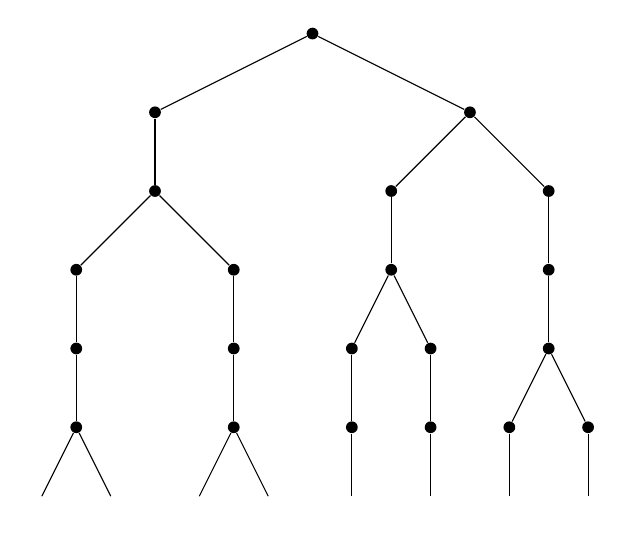
\begin{tikzpicture}

\node[] (b0) at (0,1) {};
\node[] (b1) at (1,1) {};
\node[] (b2) at (2,1) {};
\node[] (b3) at (3,1) {};
\node[] (b4) at (4,1) {};
\node[] (b5) at (5,1) {};
\node[] (b6) at (6,1) {};
\node[] (b7) at (7,1) {};

\node[circle, fill=black, inner sep=1.5pt, label=below left:$$] (c1) at (0.5,2) {};
\node[circle, fill=black, inner sep=1.5pt, label=below left:$$] (c2) at (2.5,2) {};
\node[circle, fill=black, inner sep=1.5pt, label=below left:$$] (c3) at (4,2) {};
\node[circle, fill=black, inner sep=1.5pt, label=below left:$$] (c4) at (5,2) {};
\node[circle, fill=black, inner sep=1.5pt, label=below left:$$] (c5) at (6,2) {};
\node[circle, fill=black, inner sep=1.5pt, label=below left:$$] (c6) at (7,2) {};

\node[circle, fill=black, inner sep=1.5pt, label=below left:$$] (d1) at (0.5,3) {};
\node[circle, fill=black, inner sep=1.5pt, label=below left:$$] (d2) at (2.5,3) {};
\node[circle, fill=black, inner sep=1.5pt, label=below left:$$] (d3) at (4,3) {};
\node[circle, fill=black, inner sep=1.5pt, label=below left:$$] (d4) at (5,3) {};
\node[circle, fill=black, inner sep=1.5pt, label=below left:$$] (d5) at (6.5,3) {};

\node[circle, fill=black, inner sep=1.5pt, label=below left:$$] (e1) at (0.5,4) {};
\node[circle, fill=black, inner sep=1.5pt, label=below left:$$] (e2) at (2.5,4) {};
\node[circle, fill=black, inner sep=1.5pt, label=below left:$$] (e3) at (4.5,4) {};
\node[circle, fill=black, inner sep=1.5pt, label=below left:$$] (e4) at (6.5,4) {};

\node[circle, fill=black, inner sep=1.5pt, label=below left:$$] (f1) at (1.5,5) {};
\node[circle, fill=black, inner sep=1.5pt, label=below left:$$] (f2) at (4.5,5) {};
\node[circle, fill=black, inner sep=1.5pt, label=below left:$$] (f3) at (6.5,5) {};

\node[circle, fill=black, inner sep=1.5pt, label=below left:$$] (g1) at (1.5,6) {};
\node[circle, fill=black, inner sep=1.5pt, label=below left:$$] (g2) at (5.5,6) {};

\node[circle, fill=black, inner sep=1.5pt, label=below left:$$] (h1) at (3.5,7) {};

\draw (b0) -- (c1);
\draw (b1) -- (c1);
\draw (b2) -- (c2);
\draw (b3) -- (c2);
\draw (b4) -- (c3);
\draw (b5) -- (c4);
\draw (b6) -- (c5);
\draw (b7) -- (c6);

\draw (c1) -- (d1);
\draw (c2) -- (d2);
\draw (c3) -- (d3);
\draw (c4) -- (d4);
\draw (c5) -- (d5);
\draw (c6) -- (d5);

\draw (d1) -- (e1);
\draw (d2) -- (e2);
\draw (d3) -- (e3);
\draw (d4) -- (e3);
\draw (d5) -- (e4);

\draw (e1) -- (f1);
\draw (e2) -- (f1);
\draw (e3) -- (f2);
\draw (e4) -- (f3);

\draw (f1) -- (g1);
\draw (f2) -- (g2);
\draw (f3) -- (g2);

\draw (g1) -- (h1);
\draw (g2) -- (h1);

\end{tikzpicture} \end{center}

\end{example}

\begin{defn} Let $T$ be a $P$-tree on $n$ leaves $\ell_{1},\dots,\ell_{n}$.
For $i=1,2\dots,n-1$, we define the $i$'th \textbf{gap }$g_{i}$
of $T$ to be
\[
g_{i}:=\{\ell_{i},\ell_{i+1}\}.
\]

The \textbf{height }of a gap $g_{i}$ in $T$ is the height of the
greatest common ancestor of $\ell_{i}$ and $\ell_{i+1}$ in $T$.
We denote the height of a gap $g_{i}$ in $T$ as $h_{T}(g_{i})$.
\end{defn}

\subsubsection{non-degenerate $P$-trees and total preorders.}

~~~We want to show how non-degenerate $P$-trees correspond to
total preorders. First we define what a total preorder is.

\begin{defn} Let $X$ be a set. A \textbf{preorder }on $X$ is a
binary relation $\leq$ which satisfies the following properties
\begin{enumerate}
\item (reflexive) $x\leq x$ for all $x\in X$.
\item (transitive) If $x\leq y$ and $y\leq z$, then $x\leq z$ for all
$x,y,z\in X$.
\end{enumerate}
If in addition either $x\leq y$ or $y\leq x$ for all $x,y\in X$,
then we say $\leq$ is a \textbf{total preorder} on $X$. \end{defn}

\begin{defn} Let $\leq$ be a total preorder on a $X$ and let $x\in X$.
We say $x$ is a \textbf{maximal element }of $\leq$ if $y\leq x$
for every $y\in X$. \end{defn}

\begin{defn} Let $\leq$ be a total preorder on a finite set $X$
and let $x\in X$. If $x$ is a maximal element of $\le$, then we
say\textbf{ $x$ }comes in\textbf{ first} \textbf{place} under $\leq$.
Denote $X_{1}$ to be the set of all elements which comes in first
place under $\leq$, i.e. the maximal elements under $\leq$. If $x$
is a maximal element of $\leq$ restricted to $X-X_{1}$, then we
say $x$ comes in \textbf{second place }under $\leq$. Proceeding
inductively, if $x$ is a maximal element of $\leq$ restricted to
$X-X_{1}-\cdots-X_{i-1}$, then we say $x$ comes in \textbf{$i$th
place}. \end{defn}

\begin{theorem} Let $\mathcal{P}_{n}$ be the set of all non-degenerate
$P$-trees on $n+1$ leaves and let $\mathcal{T}_{n}$ be the set
of all total preorders on the set $[n]:=\{1,2,\dots,n\}$. Then $\mathcal{P}_{n}\cong\mathcal{T}_{n}$.
\end{theorem}

\begin{proof} Let $T$ be a non-degenerate $P$-tree on $n+1$ leaves.
The gaps $g_{i}$ of $T$ gives rise to a total preorder $\leq_{_{T}}$
on $[n]$: 
\[
i\leq_{_{T}}j\mbox{ if and only if }h_{T}(g_{i})\leq h_{T}(g_{j})\mbox{ for all }i,j\in[n].
\]
Conversely, if we have a total preorder on the set $[n]$, then we
can construct a $P$-tree on $n+1$ leaves whose gaps $g_{i}$ are
appropriately placed using the total preorder. \end{proof}

~~~Let $T$ be a non-degenerate $P$-tree on $n+1$ leaves and
let $\leq_{_{T}}$ be the corresponding total preorder on the set
$[n]$. Denote $\lambda_{i}$ to be the number of elements in $[n]$
which come in $i$th place under $\leq_{_{T}}$, and list these elements
in increasing order as $a_{i1},\dots,a_{i\lambda_{i}}$\footnote{By increasing order, we mean $a_{11}<\cdots<a_{1\lambda_{1}}$ where
$<$ denotes the usual order on the set $[n]$.} for $i=1,2,\dots,h_{T}$. We use the notation $(a_{11}\cdots a_{1\lambda_{1}})(a_{21}\cdots a_{2\lambda_{2}})\cdots(a_{h_{T}1}\cdots a_{h_{T}\lambda_{h_{T}}})$
to refer to this total preorder. Let us demonstrate with a few examples: 

\begin{example} The non-degenerate $P$-tree on $8$ leaves below
corresponds to the total preorder given by $(1357)(26)(5)$.

\begin{center}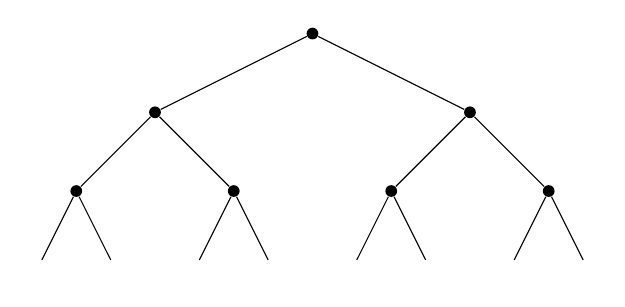
\begin{tikzpicture}

\node[] (a1) at (0,0) {};
\node[] (a2) at (1,0) {};
\node[] (a3) at (2,0) {};
\node[] (a4) at (3,0) {};
\node[] (a5) at (4,0) {};
\node[] (a6) at (5,0) {};
\node[] (a7) at (6,0) {};
\node[] (a8) at (7,0) {};

\node[circle, fill=black, inner sep=1.5pt, label=below left:$$] (b1) at (0.5,1) {};
\node[circle, fill=black, inner sep=1.5pt, label=below left:$$] (b2) at (2.5,1) {};
\node[circle, fill=black, inner sep=1.5pt, label=below left:$$] (b3) at (4.5,1) {};
\node[circle, fill=black, inner sep=1.5pt, label=below left:$$] (b4) at (6.5,1) {};

\node[circle, fill=black, inner sep=1.5pt, label=below left:$$] (c1) at (1.5,2) {};
\node[circle, fill=black, inner sep=1.5pt, label=below left:$$] (c2) at (5.5,2) {};

\node[circle, fill=black, inner sep=1.5pt, label=below left:$$] (d1) at (3.5,3) {};

\draw (a1) -- (b1);
\draw (a2) -- (b1);
\draw (a3) -- (b2);
\draw (a4) -- (b2);
\draw (a5) -- (b3);
\draw (a6) -- (b3);
\draw (a7) -- (b4);
\draw (a8) -- (b4);

\draw (b1) -- (c1);
\draw (b2) -- (c1);
\draw (b3) -- (c2);
\draw (b4) -- (c2);

\draw (c1) -- (d1);
\draw (c2) -- (d1);



\end{tikzpicture} \end{center}

\end{example}

\begin{example}The non-degenerate $P$-tree on $9$ leaves below
corresponds to the total preorder given by $(1468)(237)(5)$.

\begin{center}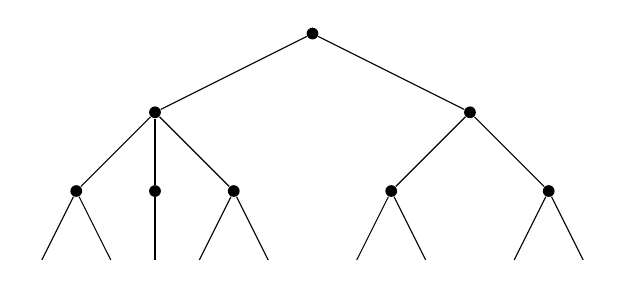
\begin{tikzpicture}

\node[] (a1) at (0,0) {};
\node[] (a2) at (1,0) {};
\node[] (a9) at (1.5,0) {};
\node[] (a3) at (2,0) {};
\node[] (a4) at (3,0) {};
\node[] (a5) at (4,0) {};
\node[] (a6) at (5,0) {};
\node[] (a7) at (6,0) {};
\node[] (a8) at (7,0) {};

\node[circle, fill=black, inner sep=1.5pt, label=below left:$$] (b1) at (0.5,1) {};
\node[circle, fill=black, inner sep=1.5pt, label=below left:$$] (b5) at (1.5,1) {};
\node[circle, fill=black, inner sep=1.5pt, label=below left:$$] (b2) at (2.5,1) {};
\node[circle, fill=black, inner sep=1.5pt, label=below left:$$] (b3) at (4.5,1) {};
\node[circle, fill=black, inner sep=1.5pt, label=below left:$$] (b4) at (6.5,1) {};


\node[circle, fill=black, inner sep=1.5pt, label=below left:$$] (c1) at (1.5,2) {};
\node[circle, fill=black, inner sep=1.5pt, label=below left:$$] (c2) at (5.5,2) {};

\node[circle, fill=black, inner sep=1.5pt, label=below left:$$] (d1) at (3.5,3) {};

\draw (a1) -- (b1);
\draw (a2) -- (b1);
\draw (a9) -- (b5);
\draw (a3) -- (b2);
\draw (a4) -- (b2);
\draw (a5) -- (b3);
\draw (a6) -- (b3);
\draw (a7) -- (b4);
\draw (a8) -- (b4);

\draw (b1) -- (c1);
\draw (b5) -- (c1);
\draw (b2) -- (c1);
\draw (b3) -- (c2);
\draw (b4) -- (c2);

\draw (c1) -- (d1);
\draw (c2) -- (d1);



\end{tikzpicture} \end{center}

\end{example}

\begin{example} The non-degenerate $P$-tree on $8$ leaves below
corresponds to the total preorder given by $(1)(3)(7)(5)(2)(6)(4)$.

\begin{center}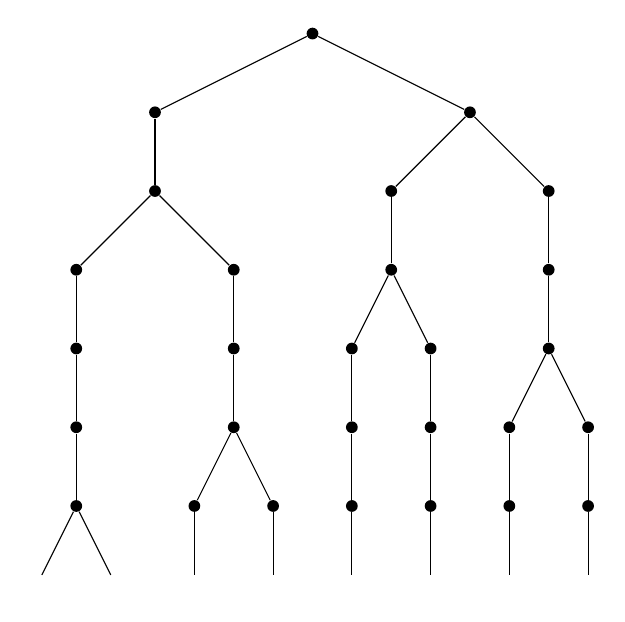
\begin{tikzpicture}

\node[] (a1) at (0,0) {};
\node[] (a2) at (1,0) {};
\node[] (a3) at (2,0) {};
\node[] (a4) at (3,0) {};
\node[] (a5) at (4,0) {};
\node[] (a6) at (5,0) {};
\node[] (a7) at (6,0) {};
\node[] (a8) at (7,0) {};

\node[circle, fill=black, inner sep=1.5pt, label=below left:$$] (b1) at (0.5,1) {};
\node[circle, fill=black, inner sep=1.5pt, label=below left:$$] (b2) at (2,1) {};
\node[circle, fill=black, inner sep=1.5pt, label=below left:$$] (b3) at (3,1) {};
\node[circle, fill=black, inner sep=1.5pt, label=below left:$$] (b4) at (4,1) {};
\node[circle, fill=black, inner sep=1.5pt, label=below left:$$] (b5) at (5,1) {};
\node[circle, fill=black, inner sep=1.5pt, label=below left:$$] (b6) at (6,1) {};
\node[circle, fill=black, inner sep=1.5pt, label=below left:$$] (b7) at (7,1) {};

\node[circle, fill=black, inner sep=1.5pt, label=below left:$$] (c1) at (0.5,2) {};
\node[circle, fill=black, inner sep=1.5pt, label=below left:$$] (c2) at (2.5,2) {};
\node[circle, fill=black, inner sep=1.5pt, label=below left:$$] (c3) at (4,2) {};
\node[circle, fill=black, inner sep=1.5pt, label=below left:$$] (c4) at (5,2) {};
\node[circle, fill=black, inner sep=1.5pt, label=below left:$$] (c5) at (6,2) {};
\node[circle, fill=black, inner sep=1.5pt, label=below left:$$] (c6) at (7,2) {};

\node[circle, fill=black, inner sep=1.5pt, label=below left:$$] (d1) at (0.5,3) {};
\node[circle, fill=black, inner sep=1.5pt, label=below left:$$] (d2) at (2.5,3) {};
\node[circle, fill=black, inner sep=1.5pt, label=below left:$$] (d3) at (4,3) {};
\node[circle, fill=black, inner sep=1.5pt, label=below left:$$] (d4) at (5,3) {};
\node[circle, fill=black, inner sep=1.5pt, label=below left:$$] (d5) at (6.5,3) {};

\node[circle, fill=black, inner sep=1.5pt, label=below left:$$] (e1) at (0.5,4) {};
\node[circle, fill=black, inner sep=1.5pt, label=below left:$$] (e2) at (2.5,4) {};
\node[circle, fill=black, inner sep=1.5pt, label=below left:$$] (e3) at (4.5,4) {};
\node[circle, fill=black, inner sep=1.5pt, label=below left:$$] (e4) at (6.5,4) {};

\node[circle, fill=black, inner sep=1.5pt, label=below left:$$] (f1) at (1.5,5) {};
\node[circle, fill=black, inner sep=1.5pt, label=below left:$$] (f2) at (4.5,5) {};
\node[circle, fill=black, inner sep=1.5pt, label=below left:$$] (f3) at (6.5,5) {};

\node[circle, fill=black, inner sep=1.5pt, label=below left:$$] (g1) at (1.5,6) {};
\node[circle, fill=black, inner sep=1.5pt, label=below left:$$] (g2) at (5.5,6) {};

\node[circle, fill=black, inner sep=1.5pt, label=below left:$$] (h1) at (3.5,7) {};


\draw (a1) -- (b1);
\draw (a2) -- (b1);
\draw (a3) -- (b2);
\draw (a4) -- (b3);
\draw (a5) -- (b4);
\draw (a6) -- (b5);
\draw (a7) -- (b6);
\draw (a8) -- (b7);

\draw (b1) -- (c1);
\draw (b2) -- (c2);
\draw (b3) -- (c2);
\draw (b4) -- (c3);
\draw (b5) -- (c4);
\draw (b6) -- (c5);
\draw (b7) -- (c6);

\draw (c1) -- (d1);
\draw (c2) -- (d2);
\draw (c3) -- (d3);
\draw (c4) -- (d4);
\draw (c5) -- (d5);
\draw (c6) -- (d5);

\draw (d1) -- (e1);
\draw (d2) -- (e2);
\draw (d3) -- (e3);
\draw (d4) -- (e3);
\draw (d5) -- (e4);

\draw (e1) -- (f1);
\draw (e2) -- (f1);
\draw (e3) -- (f2);
\draw (e4) -- (f3);

\draw (f1) -- (g1);
\draw (f2) -- (g2);
\draw (f3) -- (g2);

\draw (g1) -- (h1);
\draw (g2) -- (h1);

\end{tikzpicture} \end{center}

\end{example}

\begin{example} The non-degenerate $P$-tree on $8$ leaves below
corresponds to the total preorder given by $(13)(7)(5)(2)(6)(4)$.

\begin{center}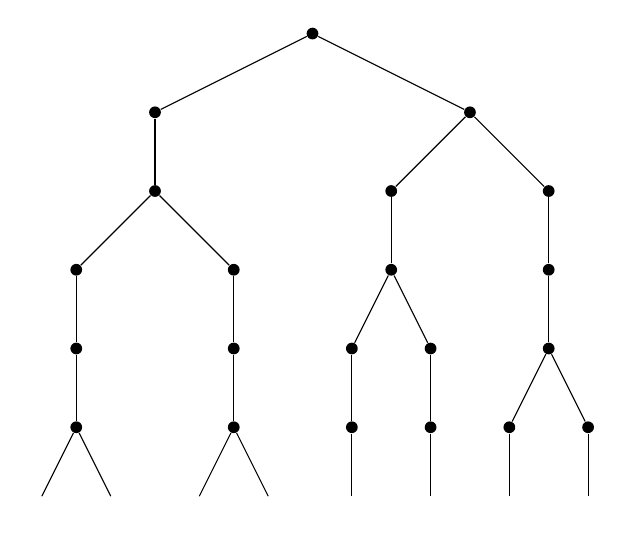
\begin{tikzpicture}

\node[] (b0) at (0,1) {};
\node[] (b1) at (1,1) {};
\node[] (b2) at (2,1) {};
\node[] (b3) at (3,1) {};
\node[] (b4) at (4,1) {};
\node[] (b5) at (5,1) {};
\node[] (b6) at (6,1) {};
\node[] (b7) at (7,1) {};

\node[circle, fill=black, inner sep=1.5pt, label=below left:$$] (c1) at (0.5,2) {};
\node[circle, fill=black, inner sep=1.5pt, label=below left:$$] (c2) at (2.5,2) {};
\node[circle, fill=black, inner sep=1.5pt, label=below left:$$] (c3) at (4,2) {};
\node[circle, fill=black, inner sep=1.5pt, label=below left:$$] (c4) at (5,2) {};
\node[circle, fill=black, inner sep=1.5pt, label=below left:$$] (c5) at (6,2) {};
\node[circle, fill=black, inner sep=1.5pt, label=below left:$$] (c6) at (7,2) {};

\node[circle, fill=black, inner sep=1.5pt, label=below left:$$] (d1) at (0.5,3) {};
\node[circle, fill=black, inner sep=1.5pt, label=below left:$$] (d2) at (2.5,3) {};
\node[circle, fill=black, inner sep=1.5pt, label=below left:$$] (d3) at (4,3) {};
\node[circle, fill=black, inner sep=1.5pt, label=below left:$$] (d4) at (5,3) {};
\node[circle, fill=black, inner sep=1.5pt, label=below left:$$] (d5) at (6.5,3) {};

\node[circle, fill=black, inner sep=1.5pt, label=below left:$$] (e1) at (0.5,4) {};
\node[circle, fill=black, inner sep=1.5pt, label=below left:$$] (e2) at (2.5,4) {};
\node[circle, fill=black, inner sep=1.5pt, label=below left:$$] (e3) at (4.5,4) {};
\node[circle, fill=black, inner sep=1.5pt, label=below left:$$] (e4) at (6.5,4) {};

\node[circle, fill=black, inner sep=1.5pt, label=below left:$$] (f1) at (1.5,5) {};
\node[circle, fill=black, inner sep=1.5pt, label=below left:$$] (f2) at (4.5,5) {};
\node[circle, fill=black, inner sep=1.5pt, label=below left:$$] (f3) at (6.5,5) {};

\node[circle, fill=black, inner sep=1.5pt, label=below left:$$] (g1) at (1.5,6) {};
\node[circle, fill=black, inner sep=1.5pt, label=below left:$$] (g2) at (5.5,6) {};

\node[circle, fill=black, inner sep=1.5pt, label=below left:$$] (h1) at (3.5,7) {};

\draw (b0) -- (c1);
\draw (b1) -- (c1);
\draw (b2) -- (c2);
\draw (b3) -- (c2);
\draw (b4) -- (c3);
\draw (b5) -- (c4);
\draw (b6) -- (c5);
\draw (b7) -- (c6);

\draw (c1) -- (d1);
\draw (c2) -- (d2);
\draw (c3) -- (d3);
\draw (c4) -- (d4);
\draw (c5) -- (d5);
\draw (c6) -- (d5);

\draw (d1) -- (e1);
\draw (d2) -- (e2);
\draw (d3) -- (e3);
\draw (d4) -- (e3);
\draw (d5) -- (e4);

\draw (e1) -- (f1);
\draw (e2) -- (f1);
\draw (e3) -- (f2);
\draw (e4) -- (f3);

\draw (f1) -- (g1);
\draw (f2) -- (g2);
\draw (f3) -- (g2);

\draw (g1) -- (h1);
\draw (g2) -- (h1);

\end{tikzpicture} \end{center}

\end{example}

\begin{example} The non-degenerate $P$-tree on $8$ leaves below
corresponds to the total preorder given by $(3)(1)(7)(5)(2)(6)(4)$.

\begin{center}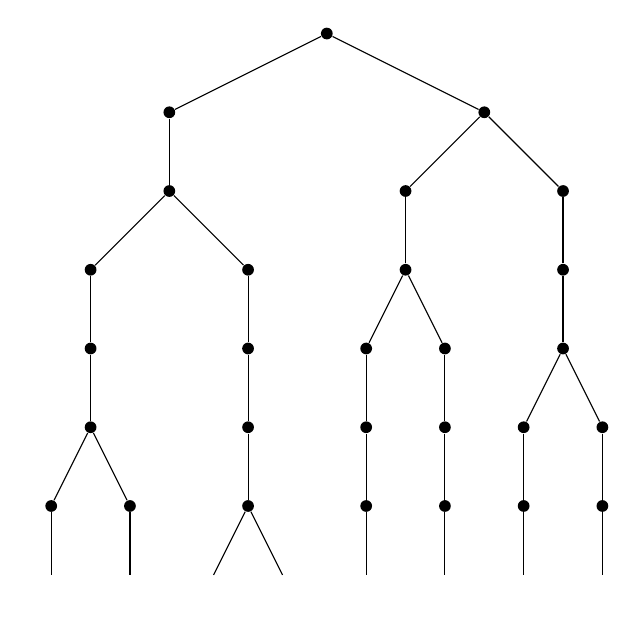
\begin{tikzpicture}

\node[] (a1) at (0,0) {};
\node[] (a2) at (1,0) {};
\node[] (a3) at (2,0) {};
\node[] (a4) at (3,0) {};
\node[] (a5) at (4,0) {};
\node[] (a6) at (5,0) {};
\node[] (a7) at (6,0) {};
\node[] (a8) at (7,0) {};

\node[circle, fill=black, inner sep=1.5pt, label=below left:$$] (b1) at (0,1) {};
\node[circle, fill=black, inner sep=1.5pt, label=below left:$$] (b2) at (1,1) {};
\node[circle, fill=black, inner sep=1.5pt, label=below left:$$] (b3) at (2.5,1) {};
\node[circle, fill=black, inner sep=1.5pt, label=below left:$$] (b4) at (4,1) {};
\node[circle, fill=black, inner sep=1.5pt, label=below left:$$] (b5) at (5,1) {};
\node[circle, fill=black, inner sep=1.5pt, label=below left:$$] (b6) at (6,1) {};
\node[circle, fill=black, inner sep=1.5pt, label=below left:$$] (b7) at (7,1) {};

\node[circle, fill=black, inner sep=1.5pt, label=below left:$$] (c1) at (0.5,2) {};
\node[circle, fill=black, inner sep=1.5pt, label=below left:$$] (c2) at (2.5,2) {};
\node[circle, fill=black, inner sep=1.5pt, label=below left:$$] (c3) at (4,2) {};
\node[circle, fill=black, inner sep=1.5pt, label=below left:$$] (c4) at (5,2) {};
\node[circle, fill=black, inner sep=1.5pt, label=below left:$$] (c5) at (6,2) {};
\node[circle, fill=black, inner sep=1.5pt, label=below left:$$] (c6) at (7,2) {};

\node[circle, fill=black, inner sep=1.5pt, label=below left:$$] (d1) at (0.5,3) {};
\node[circle, fill=black, inner sep=1.5pt, label=below left:$$] (d2) at (2.5,3) {};
\node[circle, fill=black, inner sep=1.5pt, label=below left:$$] (d3) at (4,3) {};
\node[circle, fill=black, inner sep=1.5pt, label=below left:$$] (d4) at (5,3) {};
\node[circle, fill=black, inner sep=1.5pt, label=below left:$$] (d5) at (6.5,3) {};

\node[circle, fill=black, inner sep=1.5pt, label=below left:$$] (e1) at (0.5,4) {};
\node[circle, fill=black, inner sep=1.5pt, label=below left:$$] (e2) at (2.5,4) {};
\node[circle, fill=black, inner sep=1.5pt, label=below left:$$] (e3) at (4.5,4) {};
\node[circle, fill=black, inner sep=1.5pt, label=below left:$$] (e4) at (6.5,4) {};

\node[circle, fill=black, inner sep=1.5pt, label=below left:$$] (f1) at (1.5,5) {};
\node[circle, fill=black, inner sep=1.5pt, label=below left:$$] (f2) at (4.5,5) {};
\node[circle, fill=black, inner sep=1.5pt, label=below left:$$] (f3) at (6.5,5) {};

\node[circle, fill=black, inner sep=1.5pt, label=below left:$$] (g1) at (1.5,6) {};
\node[circle, fill=black, inner sep=1.5pt, label=below left:$$] (g2) at (5.5,6) {};

\node[circle, fill=black, inner sep=1.5pt, label=below left:$$] (h1) at (3.5,7) {};


\draw (a1) -- (b1);
\draw (a2) -- (b2);
\draw (a3) -- (b3);
\draw (a4) -- (b3);
\draw (a5) -- (b4);
\draw (a6) -- (b5);
\draw (a7) -- (b6);
\draw (a8) -- (b7);

\draw (b1) -- (c1);
\draw (b2) -- (c1);
\draw (b3) -- (c2);
\draw (b4) -- (c3);
\draw (b5) -- (c4);
\draw (b6) -- (c5);
\draw (b7) -- (c6);

\draw (c1) -- (d1);
\draw (c2) -- (d2);
\draw (c3) -- (d3);
\draw (c4) -- (d4);
\draw (c5) -- (d5);
\draw (c6) -- (d5);

\draw (d1) -- (e1);
\draw (d2) -- (e2);
\draw (d3) -- (e3);
\draw (d4) -- (e3);
\draw (d5) -- (e4);

\draw (e1) -- (f1);
\draw (e2) -- (f1);
\draw (e3) -- (f2);
\draw (e4) -- (f3);

\draw (f1) -- (g1);
\draw (f2) -- (g2);
\draw (f3) -- (g2);

\draw (g1) -- (h1);
\draw (g2) -- (h1);

\end{tikzpicture} \end{center}

\end{example}

~~~Let $T$ be a non-degenerate $P$-tree on $n+1$ leaves and
let $(a_{11}\cdots a_{1\lambda_{1}})(a_{21}\cdots a_{2\lambda_{2}})\cdots(a_{h_{T}1}\cdots a_{h_{T}\lambda_{h_{T}}})$
be its corresponding total preorder on $[n]$. Fix $i\in\{1,\dots,h_{T}\}$.
For $j\in\{1,\dots,\lambda_{i}\}$, we say $a_{ij}$ and $a_{i(j+1)}$
are $T$-\textbf{consecutive }if for every $a_{rs}$ where $i<r\leq h_{T}$
and $1\leq s\leq\lambda_{r}$, either $a_{rs}<a_{ij}$ or $a_{i(j+1)}<a_{rs}$.
We denote $[a_{ij}a_{i(j+1)}\cdots a_{i(j+m)}]$ to mean $a_{i(j+k)}$
and $a_{i(j+k+1)}$ are $T$-consecutive for every $0\leq k<m\leq\lambda_{i}$,
and we call it a $T$-\textbf{consecutive sequence} \textbf{of} \textbf{length
$m$}. By counting $T$-consecutive sequences and their corresponding
lengths, we obtain a complete picture of the branching nodes at height
$h_{T}-i$. Maximal $T$-consecutive sequences give rise to a partition
of the set $(a_{i1}\cdots a_{i\lambda_{i}})$ as follows: Write 
\[
(a_{i1}\cdots a_{i\lambda_{i}})=([a_{i1}\cdots a_{im_{1}}][a_{i(m_{1}+1)}\cdots a_{im_{2}}]\cdots[a_{i(m_{i}+1)}\cdots a_{i\lambda_{i}}]),
\]
where $1\leq m_{1}\leq m_{2}\cdots\leq m_{i}\leq\lambda_{i}$, and
$a_{im_{k}}$ is not $T$-consecutive to $a_{im_{k+1}}$ for all $1\leq k\leq i$.
This tells us that there are $m_{i}$ branching nodes at height $h_{T}-i$.
Writing the nodes from left to right as $n_{1},\dots,n_{m_{i}}$,
the corresponding number of children for each node is then $m_{1}+1,\dots,m_{i}+1$. 

\begin{example} Let $T$ be the non-degenerate $P$-tree on $17$
leaves whose corresponding total preorder is given by $(3\,5\,6\,8\,10\,12\,14)(1\,2\,4\,7\,11\,15\,16)(9\,13)$.
Let's decompose this into its $T$-consecutive parts:
\[
(3\,5\,6\,8\,10\,12\,14)(1\,2\,4\,7\,11\,15\,16)(9\,13)=([3][5\,6][8][10][12][14])([1\,2\,4\,7][11][15\,16])([9\,13])
\]

At height $2$, there are $6$ branching nodes, and the number of
children associated to each branching node from left to right is $2,3,2,2,2,2$.
At height $1$, there are $3$ branching nodes, and the number of
children associated to each branching from left to right is $5,2,3$.
At height $0$, there is only one branching node, i.e. the root, and
it has $3$ children: 

\begin{center}\begin{tikzpicture}

\node[] (a1) at (0,0) {};
\node[] (a2) at (1,0) {};
\node[] (a3) at (2,0) {};
\node[] (a4) at (3,0) {};
\node[] (a5) at (4,0) {};
\node[] (a6) at (5,0) {};
\node[] (a7) at (6,0) {};
\node[] (a8) at (7,0) {};
\node[] (a9) at (8,0) {};
\node[] (a10) at (9,0) {};
\node[] (a11) at (10,0) {};
\node[] (a12) at (11,0) {};
\node[] (a13) at (12,0) {};
\node[] (a14) at (13,0) {};
\node[] (a15) at (14,0) {};
\node[] (a16) at (15,0) {};
\node[] (a17) at (16,0) {};


\node[circle, fill=black, inner sep=1.5pt, label=below left:$$] (b1) at (0,2) {};
\node[circle, fill=black, inner sep=1.5pt, label=below left:$$] (b2) at (1,2) {};
\node[circle, fill=black, inner sep=1.5pt, label=below left:$$] (b3) at (2.5,2) {};
\node[circle, fill=black, inner sep=1.5pt, label=below left:$$] (b4) at (5,2) {};
\node[circle, fill=black, inner sep=1.5pt, label=below left:$$] (b5) at (7.5,2) {};
\node[circle, fill=black, inner sep=1.5pt, label=below left:$$] (b6) at (9.5,2) {};
\node[circle, fill=black, inner sep=1.5pt, label=below left:$$] (b7) at (11.5,2) {};
\node[circle, fill=black, inner sep=1.5pt, label=below left:$$] (b8) at (13.5,2) {};
\node[circle, fill=black, inner sep=1.5pt, label=below left:$$] (b9) at (15,2) {};
\node[circle, fill=black, inner sep=1.5pt, label=below left:$$] (b10) at (16,2) {};

\node[circle, fill=black, inner sep=1.5pt, label=below left:$$] (c1) at (3,4) {};
\node[circle, fill=black, inner sep=1.5pt, label=below left:$$] (c2) at (10.5,4) {};
\node[circle, fill=black, inner sep=1.5pt, label=below left:$$] (c3) at (15,4) {};

\node[circle, fill=black, inner sep=1.5pt, label=below left:$$] (d1) at (8,6) {};


\draw (a1) -- (b1);
\draw (a2) -- (b2);
\draw (a3) -- (b3);
\draw (a4) -- (b3);
\draw (a5) -- (b4);
\draw (a6) -- (b4);
\draw (a7) -- (b4);
\draw (a8) -- (b5);
\draw (a9) -- (b5);
\draw (a10) -- (b6);
\draw (a11) -- (b6);
\draw (a12) -- (b7);
\draw (a13) -- (b7);
\draw (a14) -- (b8);
\draw (a15) -- (b8);
\draw (a16) -- (b9);
\draw (a17) -- (b10);

\draw (b1) -- (c1);
\draw (b2) -- (c1);
\draw (b3) -- (c1);
\draw (b4) -- (c1);
\draw (b5) -- (c1);
\draw (b6) -- (c2);
\draw (b7) -- (c2);
\draw (b8) -- (c3);
\draw (b9) -- (c3);
\draw (b10) -- (c3);

\draw (c1) -- (d1);
\draw (c2) -- (d1);
\draw (c3) -- (d1);

\end{tikzpicture} \end{center}

\end{example}

\subsection{$P$-tree polynomial}

~~~Let $\mathcal{P}$ be the set of all $P$-trees. Define a map
$\varphi:\mathcal{P}\to\mathbb{Z}[x]$, denoted $T\mapsto\varphi_{T}(x)$,
as follows: given a $P$-tree $T$ on $n$-leaves $\ell_{1},\dots,\ell_{n}$,
assign the value $1$ to $\ell_{i}$ for each $1\leq i\leq n$. If
a node has two or more children, then assign to it the sum of the
values assigned to each child. If a node has only one child, then
assign to it the value of its child multiplied by $x$. If we do this
to each node in $T$, we will get a polynomial assigned to the root.
We set $\varphi_{T}(x)$ to be this polynomial.

\begin{example} Let $T$ be the $P$-tree corresponding to $(3)(1)(7)(5)(2)(6)(4)$.
Then $\varphi_{T}(x)=8x^{4}$. 

\begin{center}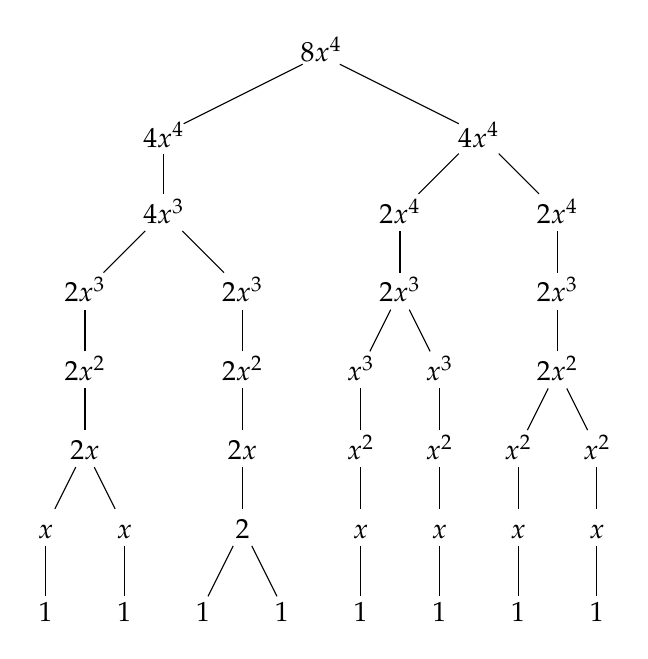
\begin{tikzpicture}

\node[label={[label distance=-0.45cm]90:$1$}] (a1) at (0,0) {};
\node[label={[label distance=-0.45cm]90:$1$}] (a2) at (1,0) {};
\node[label={[label distance=-0.45cm]90:$1$}] (a3) at (2,0) {};
\node[label={[label distance=-0.45cm]90:$1$}] (a4) at (3,0) {};
\node[label={[label distance=-0.45cm]90:$1$}] (a5) at (4,0) {};
\node[label={[label distance=-0.45cm]90:$1$}] (a6) at (5,0) {};
\node[label={[label distance=-0.45cm]90:$1$}] (a7) at (6,0) {};
\node[label={[label distance=-0.45cm]90:$1$}] (a8) at (7,0) {};

\node[label={[label distance=-0.5cm]90:$x$}, inner sep=6.5pt] (b1) at (0,1) {};
\node[label={[label distance=-0.5cm]90:$x$}, inner sep=6.5pt] (b2) at (1,1) {};
\node[label={[label distance=-0.5cm]90:$2$}, inner sep=6.5pt] (b3) at (2.5,1) {};
\node[label={[label distance=-0.5cm]90:$x$}, inner sep=6.5pt] (b4) at (4,1) {};
\node[label={[label distance=-0.5cm]90:$x$}, inner sep=6.5pt] (b5) at (5,1) {};
\node[label={[label distance=-0.5cm]90:$x$}, inner sep=6.5pt] (b6) at (6,1) {};
\node[label={[label distance=-0.5cm]90:$x$}, inner sep=6.5pt] (b7) at (7,1) {};

\node[label={[label distance=-0.5cm]90:$2x$}, inner sep=6.5pt] (c1) at (0.5,2) {};
\node[label={[label distance=-0.5cm]90:$2x$}, inner sep=6.5pt] (c2) at (2.5,2) {};
\node[label={[label distance=-0.5cm]90:$x^2 $}, inner sep=6.5pt] (c3) at (4,2) {};
\node[label={[label distance=-0.5cm]90:$x^2 $}, inner sep=6.5pt] (c4) at (5,2) {};
\node[label={[label distance=-0.5cm]90:$x^2 $}, inner sep=6.5pt] (c5) at (6,2) {};
\node[label={[label distance=-0.5cm]90:$x^2 $}, inner sep=6.5pt] (c6) at (7,2) {};

\node[label={[label distance=-0.5cm]90:$2x^2 $}, inner sep=6.5pt] (d1) at (0.5,3) {};
\node[label={[label distance=-0.5cm]90:$2x^2 $}, inner sep=6.5pt] (d2) at (2.5,3) {};
\node[label={[label distance=-0.5cm]90:$x^3 $}, inner sep=6.5pt] (d3) at (4,3) {};
\node[label={[label distance=-0.5cm]90:$x^3 $}, inner sep=6.5pt] (d4) at (5,3) {};
\node[label={[label distance=-0.5cm]90:$2x^2 $}, inner sep=6.5pt] (d5) at (6.5,3) {};

\node[label={[label distance=-0.5cm]90:$2x^3 $}, inner sep=6.5pt] (e1) at (0.5,4) {};
\node[label={[label distance=-0.5cm]90:$2x^3 $}, inner sep=6.5pt] (e2) at (2.5,4) {};
\node[label={[label distance=-0.5cm]90:$2x^3 $}, inner sep=6.5pt] (e3) at (4.5,4) {};
\node[label={[label distance=-0.5cm]90:$2x^3 $}, inner sep=6.5pt] (e4) at (6.5,4) {};

\node[label={[label distance=-0.5cm]90:$4x^3 $}, inner sep=6.5pt] (f1) at (1.5,5) {};
\node[label={[label distance=-0.5cm]90:$2x^4 $}, inner sep=6.5pt] (f2) at (4.5,5) {};
\node[label={[label distance=-0.5cm]90:$2x^4 $}, inner sep=6.5pt] (f3) at (6.5,5) {};

\node[label={[label distance=-0.55cm]90:$4x^4 $}, inner sep=7pt] (g1) at (1.5,6) {};
\node[label={[label distance=-0.55cm]90:$4x^4 $}, inner sep=7pt] (g2) at (5.5,6) {};

\node[label={[label distance=-0.45cm]90:$8x^4 $}, inner sep=6.5pt] (h1) at (3.5,7) {};


\draw (a1) -- (b1);
\draw (a2) -- (b2);
\draw (a3) -- (b3);
\draw (a4) -- (b3);
\draw (a5) -- (b4);
\draw (a6) -- (b5);
\draw (a7) -- (b6);
\draw (a8) -- (b7);

\draw (b1) -- (c1);
\draw (b2) -- (c1);
\draw (b3) -- (c2);
\draw (b4) -- (c3);
\draw (b5) -- (c4);
\draw (b6) -- (c5);
\draw (b7) -- (c6);

\draw (c1) -- (d1);
\draw (c2) -- (d2);
\draw (c3) -- (d3);
\draw (c4) -- (d4);
\draw (c5) -- (d5);
\draw (c6) -- (d5);

\draw (d1) -- (e1);
\draw (d2) -- (e2);
\draw (d3) -- (e3);
\draw (d4) -- (e3);
\draw (d5) -- (e4);

\draw (e1) -- (f1);
\draw (e2) -- (f1);
\draw (e3) -- (f2);
\draw (e4) -- (f3);

\draw (f1) -- (g1);
\draw (f2) -- (g2);
\draw (f3) -- (g2);

\draw (g1) -- (h1);
\draw (g2) -- (h1);

\end{tikzpicture} \end{center}\end{example}

\begin{example} Let $T$ be the $P$-tree corresponding to $(1468)(237)(5)$.
Then $\varphi_{T}(x)=8+x$. 

\begin{center}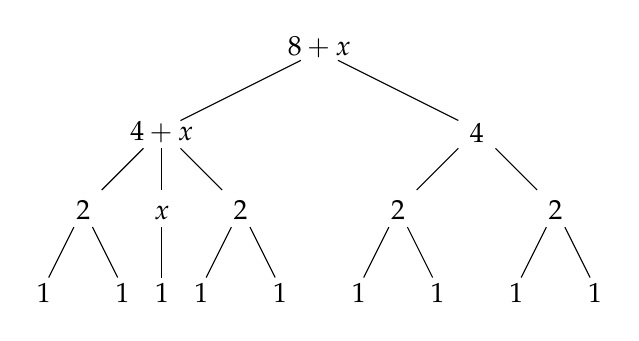
\begin{tikzpicture}

\node[label={[label distance=-0.45cm]90:$1$}] (a1) at (0,0) {};
\node[label={[label distance=-0.45cm]90:$1$}] (a2) at (1,0) {};
\node[label={[label distance=-0.45cm]90:$1$}] (a9) at (1.5,0) {};
\node[label={[label distance=-0.45cm]90:$1$}] (a3) at (2,0) {};
\node[label={[label distance=-0.45cm]90:$1$}] (a4) at (3,0) {};
\node[label={[label distance=-0.45cm]90:$1$}] (a5) at (4,0) {};
\node[label={[label distance=-0.45cm]90:$1$}] (a6) at (5,0) {};
\node[label={[label distance=-0.45cm]90:$1$}] (a7) at (6,0) {};
\node[label={[label distance=-0.45cm]90:$1$}] (a8) at (7,0) {};

\node[label={[label distance=-0.5cm]90:$2$}, inner sep=6.5pt] (b1) at (0.5,1) {};
\node[label={[label distance=-0.5cm]90:$x$}, inner sep=6.5pt] (b5) at (1.5,1) {};
\node[label={[label distance=-0.5cm]90:$2$}, inner sep=6.5pt] (b2) at (2.5,1) {};
\node[label={[label distance=-0.5cm]90:$2$}, inner sep=6.5pt] (b3) at (4.5,1) {};
\node[label={[label distance=-0.5cm]90:$2$}, inner sep=6.5pt] (b4) at (6.5,1) {};


\node[label={[label distance=-0.52cm]90:$4+x$}, inner sep=6.5pt] (c1) at (1.5,2) {};
\node[label={[label distance=-0.52cm]90:$4$}, inner sep=6.5pt] (c2) at (5.5,2) {};

\node[label={[label distance=-0.45cm]90:$8+x$}, inner sep=6.5pt] (d1) at (3.5,3) {};

\draw (a1) -- (b1);
\draw (a2) -- (b1);
\draw (a9) -- (b5);
\draw (a3) -- (b2);
\draw (a4) -- (b2);
\draw (a5) -- (b3);
\draw (a6) -- (b3);
\draw (a7) -- (b4);
\draw (a8) -- (b4);

\draw (b1) -- (c1);
\draw (b5) -- (c1);
\draw (b2) -- (c1);
\draw (b3) -- (c2);
\draw (b4) -- (c2);

\draw (c1) -- (d1);
\draw (c2) -- (d1);



\end{tikzpicture} \end{center}

\end{example}

~~~Let $T$ be a $P$-tree with root $r$ and let $v_{1},\dots,v_{k}$
be the children of $r$. Let $T_{1},\dots,T_{k}$ be the subtrees
of $T$ such that $v_{i}$ is the root of $T_{i}$ for $i=1,2\dots,k$.
It is not necessarily true that the $T_{i}$ are $P$-trees; there
may be degenerate levels, but it turns out that we can always move
the degenerate levels to the bottom. This is because for all $f,g\in\mathbb{Z}[x]$,
we have $x(f+g)=xf+xg$. We can visualize this identity in terms of
trees:

\begin{center}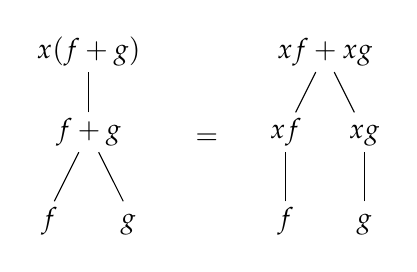
\begin{tikzpicture}

\node[label={[label distance=-0.55cm]90:$f$}] (a1) at (0,0) {};
\node[label={[label distance=-0.55cm]90:$g$}] (a2) at (1,0) {};
\node[label={[label distance=-0.55cm]90:$f$}] (a3) at (3,0) {};
\node[label={[label distance=-0.55cm]90:$g$}] (a4) at (4,0) {};

\node[label={[label distance=-0.55cm]90:$f + g$}, inner sep=7pt] (b1) at (0.5,1) {};
\node[label={[label distance=-0.55cm]90:$xf$}, inner sep=7pt] (b2) at (3,1) {};
\node[label={[label distance=-0.55cm]90:$xg$}, inner sep=7pt] (b3) at (4,1) {};


\node[label={[label distance=-0.52cm]90:$x(f+g)$}, inner sep=6.5pt] (c1) at (0.5,2) {};
\node[label={[label distance=-0.52cm]90:$xf+ xg$}, inner sep=6.5pt] (c2) at (3.5,2) {};

\node[label={$=$}] (a) at (2,0.6) {};


\draw (a1) -- (b1);
\draw (a2) -- (b1);
\draw (a3) -- (b2);
\draw (a4) -- (b3);

\draw (b1) -- (c1);
\draw (b2) -- (c2);
\draw (b3) -- (c2);



\end{tikzpicture} \end{center}

So each tree $T_{i}$ can be thought of as a $P$-tree $\tilde{T}_{i}$
with some degenerate levels attached to the bottom. With this in mind,
we arrive at the following identity:
\begin{equation}
\varphi_{T}(x)=\sum_{i=1}^{k}\varphi_{\tilde{T}_{i}}(x)x^{h_{T}-h_{\tilde{T}_{i}}-1}.\label{eq:ptreepolynomial}
\end{equation}

Using (\ref{eq:ptreepolynomial}), we can prove many things about
$P$-trees using induction on the height of the root. For instance, 

\subsubsection{k-ary trees}

\begin{defn} Let $T$ be a $P$-tree. We say $T$ is $(1,k)$-\textbf{ary
}if every node which isn't a leaf has either $k$ children or $1$
child. \end{defn}

\begin{example} Here's a $(1,3)$-ary $P$-tree:

\begin{center}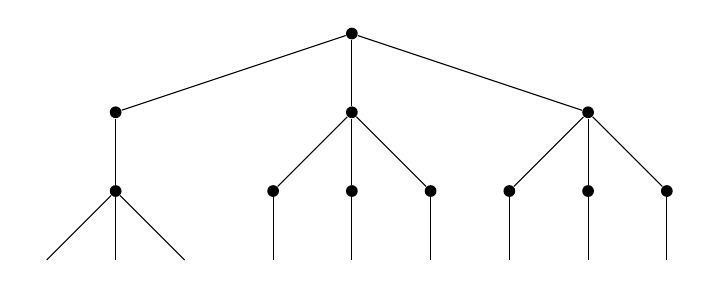
\begin{tikzpicture}

\node[] (a1) at (0,0) {};
\node[] (a2) at (1,0) {};
\node[] (a3) at (2,0) {};
\node[] (a4) at (3,0) {};
\node[] (a5) at (4,0) {};
\node[] (a6) at (5,0) {};
\node[] (a7) at (6,0) {};
\node[] (a8) at (7,0) {};
\node[] (a9) at (8,0) {};

\node[circle, fill=black, inner sep=1.5pt, label=below left:$$] (b1) at (1,1) {};
\node[circle, fill=black, inner sep=1.5pt, label=below left:$$] (b2) at (3,1) {};
\node[circle, fill=black, inner sep=1.5pt, label=below left:$$] (b3) at (4,1) {};
\node[circle, fill=black, inner sep=1.5pt, label=below left:$$] (b4) at (5,1) {};
\node[circle, fill=black, inner sep=1.5pt, label=below left:$$] (b5) at (6,1) {};
\node[circle, fill=black, inner sep=1.5pt, label=below left:$$] (b6) at (7,1) {};
\node[circle, fill=black, inner sep=1.5pt, label=below left:$$] (b7) at (8,1) {};

\node[circle, fill=black, inner sep=1.5pt, label=below left:$$] (c1) at (1,2) {};
\node[circle, fill=black, inner sep=1.5pt, label=below left:$$] (c2) at (4,2) {};
\node[circle, fill=black, inner sep=1.5pt, label=below left:$$] (c3) at (7,2) {};

\node[circle, fill=black, inner sep=1.5pt, label=below left:$$] (d1) at (4,3) {};

\draw (a1) -- (b1);
\draw (a2) -- (b1);
\draw (a3) -- (b1);
\draw (a4) -- (b2);
\draw (a5) -- (b3);
\draw (a6) -- (b4);
\draw (a7) -- (b5);
\draw (a8) -- (b6);
\draw (a9) -- (b7);

\draw (b1) -- (c1);
\draw (b2) -- (c2);
\draw (b3) -- (c2);
\draw (b4) -- (c2);
\draw (b5) -- (c3);
\draw (b6) -- (c3);
\draw (b7) -- (c3);

\draw (c1) -- (d1);
\draw (c2) -- (d1);
\draw (c3) -- (d1);

\end{tikzpicture} \end{center}

\end{example}

\begin{theorem}\label{karytree} Let $T$ be a $(1,k)$-ary $P$-tree.
Then $\varphi_{T}(k)=k^{h_{T}}$. \end{theorem}

\begin{proof} We prove this by induction on the height of a $(1,k)$-ary
$P$-tree. Suppose $T$ is a $(1,k)$-ary $P$-tree with $h_{T}=1$.
Then the root of $T$ either has one child or $k$ children. If the
root has one child, then $\varphi_{T}(x)=x$. Therefore, $\varphi_{T}(k)=k$.
If the root has $k$ children, then $\varphi_{T}(x)=k$. Therefore
the base case is true. Now assume for all $(1,k)$-ary $P$-trees
$T$ with $h_{T}\leq n$, we have $\varphi_{T}(k)=k^{h_{T}}$. Suppose
$T$ is a $(1,k)$-ary tree with $h_{T}=n+1$ and denote the root
of $T$ as $r$. 

\hfill

\textbf{Case 1}: Suppose $r$ has one child. Denote the child of $r$
as $v$ and $\tilde{T}$ as the subtree of $T$ whose root is $v$.
Then $\tilde{T}$ has height $n$ and $\varphi_{T}=x\varphi_{\tilde{T}}$.
Therefore
\begin{align*}
\varphi_{T}(k) & =k\varphi_{\tilde{T}}(k)\\
 & =k\cdot k^{n}\\
 & =k^{n+1}.
\end{align*}

\hfill

\textbf{Case 2}: Suppose $r$ has $k$ children. Denote $v_{1},\dots,v_{k}$
the children of $r$ and $T_{1},\dots,T_{k}$ the subtrees of $T$
such that the root of $T_{i}$ is $v_{i}$ for all $1\leq i\leq k$.
Then $T_{i}$ has height $n$ for all $1\leq i\leq k$ and $\varphi_{T}=\varphi_{T_{1}}+\cdots+\varphi_{T_{k}}$.
Therefore
\begin{align*}
\varphi_{T}(k) & =\varphi_{T_{1}}(k)+\cdots+\varphi_{T_{k}}(k)\\
 & =k^{n}+\cdots+k^{n}\\
 & =k\cdot k^{n}\\
 & =k^{n+1}.
\end{align*}

\end{proof}

\begin{rem} Intuitively, when we set $x=k$, we are ``splitting''
the stretching nodes into branching nodes with $k$ children: 

\begin{center}\begin{tikzpicture}

\node (a1) at (0,0) {};
\node (a2) at (2,0) {};
\node (a3) at (3,0) {};
\node (a4) at (5,0) {};

\node[circle, fill=black, inner sep=1.5pt, label=below left:$$] (b1) at (0,1) {};
\node[circle, fill=black, inner sep=1.5pt, label=below left:$$] (b2) at (3.5,1) {};



\node[label={$ \to $}] (x) at (1.2,0.2) {};
\node[label={$ \cdots $}] (y) at (3.7,0.1) {};


\draw (a1) -- (b1);
\draw (a2) -- (b2);
\draw (a3) -- (b2);
\draw (a4) -- (b2);


\end{tikzpicture} \end{center}

\end{rem}

\begin{theorem} Let $T$ be a $P$-tree. The coefficient $c_{m}$
of $x^{m}$ in $\varphi_{T}$ counts the number of root-to-leaf paths
which pass through $m$ nodes with one child. \end{theorem}

\begin{proof} We prove this by induction on the height of a $P$-tree.
Suppose $T$ is a $P$-tree with $h_{T}=1$. Then the root of $T$
either has one child or $k$ children where $k\geq1$. If the root
has one child, then $\varphi_{T}(x)=x$. There is only one root-to-leaf
path. This path passes through exactly one node with one child, namely
the root itself. If the root has $k$ children where $k\geq1$, then
$\varphi_{T}(x)=k$. There are $k$ root-to-leaf paths, all of them
pass through zero nodes with one child. Therefore the base case is
true. Now assume the statement in the theorem is true for all $P$
trees $T$ with $h_{T}\leq n$. Suppose $T$ is a $P$-tree with $h_{T}=n+1$
and denote the root of $T$ as $r$. 

\hfill

\textbf{Case 1}: Suppose $r$ has one child. Denote the child of $r$
as $v$ and $\tilde{T}$ as the subtree of $T$ whose root is $v$.
Then $\tilde{T}$ has height $n$ and $\varphi_{T}=x\varphi_{\tilde{T}}$.
Writing the coefficient of $x^{m}$ in $\varphi_{\tilde{T}}$ as $\tilde{c}_{m}$,
then $c_{m}=\tilde{c}_{m-1}$. The number of root-to-leaf paths in
$T$ which pass through $m$ nodes with one child is the same as the
number of root-to-leaf paths in $\tilde{T}$ which pass through $m-1$
nodes with one child, since the root of $T$ adds an extra node with
one child to every root-to-leaf path in $\tilde{T}$. Therefore the
statement is true in this case. 

\hfill

\textbf{Case 2}: Suppose $r$ has $k$ children. Denote $v_{1},\dots,v_{k}$
the children of $r$ and $T_{1},\dots,T_{k}$ the subtrees of $T$
such that the root of $T_{i}$ is $v_{i}$ for all $1\leq i\leq k$.
Then $T_{i}$ has height $n$ for all $1\leq i\leq k$ and $\varphi_{T}=\varphi_{T_{1}}+\cdots+\varphi_{T_{k}}$.
Writing the coefficient of $x^{m}$ in $\varphi_{T_{i}}$ as $c_{m,i}$,
then $c_{m}=c_{m,1}+\cdots+c_{m,k}$. The number of root-to-leaf paths
in $T$ which pass through $m$ nodes with one child is the same as
the number of root-to-leaf paths in $T_{1}$ which pass through $m$
nodes with one child, plus the number of root-to-leaf paths in $T_{2}$
which pass through $m$ nodes with one child, etc..., since the root
of $T$ does not add an extra node with one child to any root-to-leaf
path in $T_{i}$ for $1\leq i\leq k$. Therefore the statement is
true in this case too.

\end{proof}

\subsubsection{Symmetric Group Action}

~~~The correspondence between total preorders and $P$-trees allows
us to define an action of the symmetric group on the set of $P$-trees:
Let $T$ be a $P$-tree on $n+1$ leaves and let $(x_{11}\cdots x_{1\lambda_{1}})(x_{21}\cdots x_{2\lambda_{2}})\cdots(x_{k1}\cdots x_{k\lambda_{k}})$
be the corresponding total preorder on $[n]$. For $\sigma\in S_{n}$,
set $\sigma\cdot T$ to be the $P$-tree which corresponds to the
total preorder $(\sigma(x_{11})\cdots\sigma(x_{1\lambda_{1}}))(\sigma(x_{21})\cdots\sigma(x_{2\lambda_{2}}))\cdots(\sigma(x_{k1})\cdots\sigma(x_{k\lambda_{k}}))$. 

\subsubsection{Differential}

\begin{prop} Let $T$ be a $P$-tree with root $r$ and denote $\partial_{i}T$
to be the tree obtained from $T$ by shrinking all edges at level
$i$ to their endpoints for $i=0,1,\dots,r-1$. Then $\partial_{i}T$
is a $P$-tree. \end{prop}

\begin{proof} $\partial_{i}T$ is clearly a non-planted ordered tree.
For all nodes $v$ such that $d_{T}(v)\ge i$, we have $d_{\partial_{i}T}(v)=d_{T}(v)-1$.
In particular, for all leaves $\ell$, we have $d_{\partial_{i}T}(\ell)=d_{T}(\ell)-1$.
So all leaves have the same depth in $\partial_{i}T$. For all nodes
$v$ such that $d_{T}(v)<i$, we have $d_{\partial_{i}T}(v)=d_{T}(v)$.
So the number of nodes at height $k$ in $\partial_{i}T$ is strictly
smaller than the number of nodes at height $i-1$ in $\partial_{i}T$
for $i=1,2,\dots,r$. \end{proof}

\subsection{$A$-trees}

\begin{defn} An $A$-tree is a non-planted ordered tree which has
no nodes of degree $2$. \end{defn}

~~~There is a natural way to obtain an $A$-tree from a $P$-tree;
simply delete the nodes of degree $2$.

\begin{example} Here's the $A$-tree obtained from the $P$-tree
$(1468)(237)(5)$ by deleting a single node of degree $2$:

\begin{center}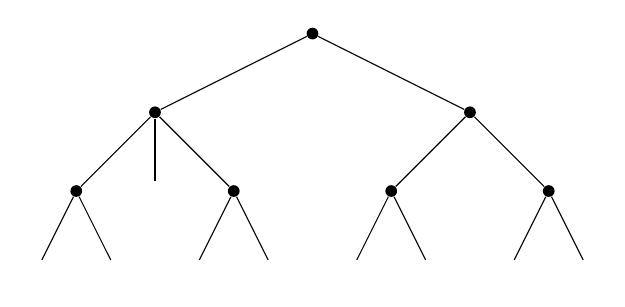
\begin{tikzpicture}

\node[] (a1) at (0,0) {};
\node[] (a2) at (1,0) {};
\node[] (a3) at (2,0) {};
\node[] (a4) at (3,0) {};
\node[] (a5) at (4,0) {};
\node[] (a6) at (5,0) {};
\node[] (a7) at (6,0) {};
\node[] (a8) at (7,0) {};

\node[circle, fill=black, inner sep=1.5pt, label=below left:$$] (b1) at (0.5,1) {};
\node[] (b5) at (1.5,1) {};
\node[circle, fill=black, inner sep=1.5pt, label=below left:$$] (b2) at (2.5,1) {};
\node[circle, fill=black, inner sep=1.5pt, label=below left:$$] (b3) at (4.5,1) {};
\node[circle, fill=black, inner sep=1.5pt, label=below left:$$] (b4) at (6.5,1) {};


\node[circle, fill=black, inner sep=1.5pt, label=below left:$$] (c1) at (1.5,2) {};
\node[circle, fill=black, inner sep=1.5pt, label=below left:$$] (c2) at (5.5,2) {};

\node[circle, fill=black, inner sep=1.5pt, label=below left:$$] (d1) at (3.5,3) {};

\draw (a1) -- (b1);
\draw (a2) -- (b1);
\draw (a3) -- (b2);
\draw (a4) -- (b2);
\draw (a5) -- (b3);
\draw (a6) -- (b3);
\draw (a7) -- (b4);
\draw (a8) -- (b4);

\draw (b1) -- (c1);
\draw (b5) -- (c1);
\draw (b2) -- (c1);
\draw (b3) -- (c2);
\draw (b4) -- (c2);

\draw (c1) -- (d1);
\draw (c2) -- (d1);



\end{tikzpicture} \end{center}

\end{example}

~~~There is a unique way to turn a $P$-tree into an $A$-tree:
simply delete the nodes of degree $2$. However there are many ways
to turn an $A$-tree into a $P$-tree. 

\section{Symmetric Group Action and the Permutohedron}

\subsection{Symmetric Group Action}

~~~The bijection between non-degenerate $P$-trees on $n+1$ leaves
and total preorders allows us to define an action of the symmetric
group on the set of non-degenerate $P$-trees on $n+1$ leaves as
follows: Let $T$ be a non-degenerate $P$-tree on $n+1$ leaves and
let $(a_{11}\cdots a_{1\lambda_{1}})(a_{21}\cdots a_{2\lambda_{2}})\cdots(a_{h_{T}1}\cdots a_{h_{T}\lambda_{k}})$
be the corresponding total preorder on $[n]$. For $\sigma\in S_{n}$,
set $\sigma\cdot T$ to be the non-degenerate $P$-tree on $n+1$
leaves whose corresponding total preorder on $[n]$ is given by $(\sigma(a_{11})\cdots\sigma(a_{1\lambda_{1}}))(\sigma(a_{21})\cdots\sigma(a_{2\lambda_{2}}))\cdots(\sigma(a_{k1})\cdots\sigma(a_{k\lambda_{k}}))$.
Using the symmetric group action, we can give a nice way to describe
every non-degenerate $P$-tree on $n+1$ leaves. Before we explain
how this works, we need some notation. 

\begin{defn} A \textbf{composition }of an integer $n$ is a sequence
$(m_{1},m_{2}\dots,m_{k})$ of strictly positive integers $m_{i}$
for $1\leq i\le k$, such that $m_{1}+m_{2}+\cdots+m_{k}=n$. \end{defn}

\begin{defn} Let $(m_{1},m_{2}\dots,m_{k})$ be a composition of
an integer $n$ and set $s_{i}=m_{1}+m_{2}+\cdots+m_{i}$ for $1\leq i\le k$.
We denote $T_{(m_{1},m_{2},\dots,m_{k})}$ to be the non-degenerate
$P$-tree on $n+1$ leaves whose corresponding total preorder on $[n]$
is given by $(1\cdots s_{1})(s_{1}+1\cdots s_{2})\cdots(s_{k-1}+1\cdots s_{k})$.
\end{defn}

\begin{example} The non-degenerate $P$-tree $T_{(3,4,2)}$ corresponds
to the total preorder on $[n]$ given by $(123)(4567)(89)$. \end{example}

\begin{defn} Let $T$ be a non-degenerate $P$-tree on $n+1$ leaves.
We denote $\mbox{Stab}(T)$ to be the stabilizer of $T$, i.e. 
\[
\mbox{Stab}(T)=\{\sigma\in S_{n}\mid\sigma\cdot T=T\}
\]
\end{defn}

\begin{example} Let $(m_{1},m_{2}\dots,m_{k})$ be a composition
of an integer $n$ and set $s_{i}=m_{1}+m_{2}+\cdots+m_{i}$ for $1\leq i\le k$.
. Then $\mbox{Stab}(T_{(m_{1},m_{2},\dots,m_{k})})$ is generated
by elementary transpositions of the form $(\ell,\ell+1)$, where $\ell\in[n]-\{s_{1},s_{2},\dots,s_{k}\}$.
\end{example}

~~~We are now ready to give a nice way to describe every non-degenerate
$P$-tree on $n+1$ leaves using the symmetric group $S_{n}$.

\begin{prop} Every non-degenerate $P$-tree on $n+1$ leaves has
the form 
\[
\overline{\sigma}\cdot T_{(m_{1},m_{2},\dots,m_{k})},
\]

where $(m_{1},m_{2},\dots m_{k})$ is a composition of $n$ and $\overline{\sigma}\in S_{n}/\mbox{Stab}(T_{(m_{1},m_{2},\dots,m_{k})})$.
\end{prop}

\begin{proof} Follows from Orbit-Stabilizer Theorem. \end{proof}

\subsection{The Permutohedron}

\begin{defn} The \textbf{permutohedron }$\mathbf{P}_{n}$\textbf{
}is the $(n-1$)-dimensional polytope in $\mathbb{R}^{n}$ defined
as the convex hull of all vectors obtained from all permutations of
the vector $(1,2\dots,n)$:
\[
\mathbf{P}_{n}:=\mbox{ConvexHull}((\sigma(1),\dots,\sigma(n))\mid\sigma\in S_{n}),
\]

where $S_{n}$ is the symmetric group. \end{defn}

~~~For each $0\leq k\leq n-1$, let $\Delta_{k}(\mathbf{P}_{n})$
be the set of $k$-cells of the $n$-dimensional permutohedron and
let $\mathcal{P}_{n}^{k}$ be the set of non-degenerate $P$-trees
on $n+1$ leaves with height $n-k$ . We construct a bijection $\Psi:\mathcal{P}_{n}^{k}\to\Delta_{k}(\mathbf{P}_{n})$
as follows: We assign $\overline{\sigma}\cdot T_{(m_{1},m_{2},\dots,m_{n-k})}$
to the $k$-cell whose center of mass is given by the coordinate 
\[
\frac{1}{m_{1}!m_{2}!\cdots m_{k}!|}\sum_{\tau\in\mbox{Stab}(T_{id,\lambda_{1},\lambda_{2},\dots,\lambda_{h_{T}}})}((\tau\sigma)^{-1}(1),(\tau\sigma)^{-1}(2),\cdots,(\tau\sigma)^{-1}(n))
\]

\begin{example} For $\sigma\in S_{n}$, the non-degenerate $P$-tree
on $n+1$ leaves given by $\overline{\sigma}\cdot T_{(1,2,\dots,n)}$
is assigned to the $0$-cell which corresponds to the coordinate $(\sigma^{-1}(1),\sigma^{-1}(2),\dots,\sigma^{-1}(n))$.
\end{example}

\section{The Associahedron}

\begin{defn} An \textbf{associahedron }$K_{n}$ is an $(n-2)$-dimensional
whose vertices correspond to binary $A$-trees on $n+1$ leaves. \end{defn}

~~~Jean-Louis Loday gave a simple formula for realizing the Stasheff
polytopes as a convex hull of integer coordinates in Euclidean space
(Loday 2004). Let $Y_{n}$ denote the set of (rooted planar) binary
trees with $n+1$ leaves (and hence $n$ internal vertices). For any
binary tree $T\in Y_{n}$, enumerate the leaves by left-to-right order,
denoted $\ell_{1},\dots,\ell_{n+1}$ and enumerate the internal vertices
as $v_{1},\dots,v_{n}$ where $v_{i}$ is the greatest common ancestor
of $\ell_{i}$ and $\ell_{i+1}$. Define a vector $M(T)\in\mathbb{R}^{n}$
whose $i$th coordinate is the product $a_{i}b_{i}$ of the number
$a_{i}$ of leaves that are left descendants of $v_{i}$ and the number
$b_{i}$ of leaves that are right descendants of $v_{i}$

\begin{theorem}. (Loday). The convex hull of the points $\{M(T)\in\mathbb{R}^{n}\mid T\in Y_{n}\}$
is a realization of the Stasheff polytope of dimension $n-1$, and
is included in the affine hyperplane $\{x_{1},\dots,x_{n}\mid x_{1}+\cdots+x_{n}=n^{2}\}$.
\end{theorem}

\section{Number of nondegenerate $P$-trees which collapse to an $A$-tree. }

The permutohedron $\mathbf{P}_{3}$ with $P$-trees on $4$ leaves
attached to each $k$-cell of $\mathbf{P}_{3}$:

\begin{center}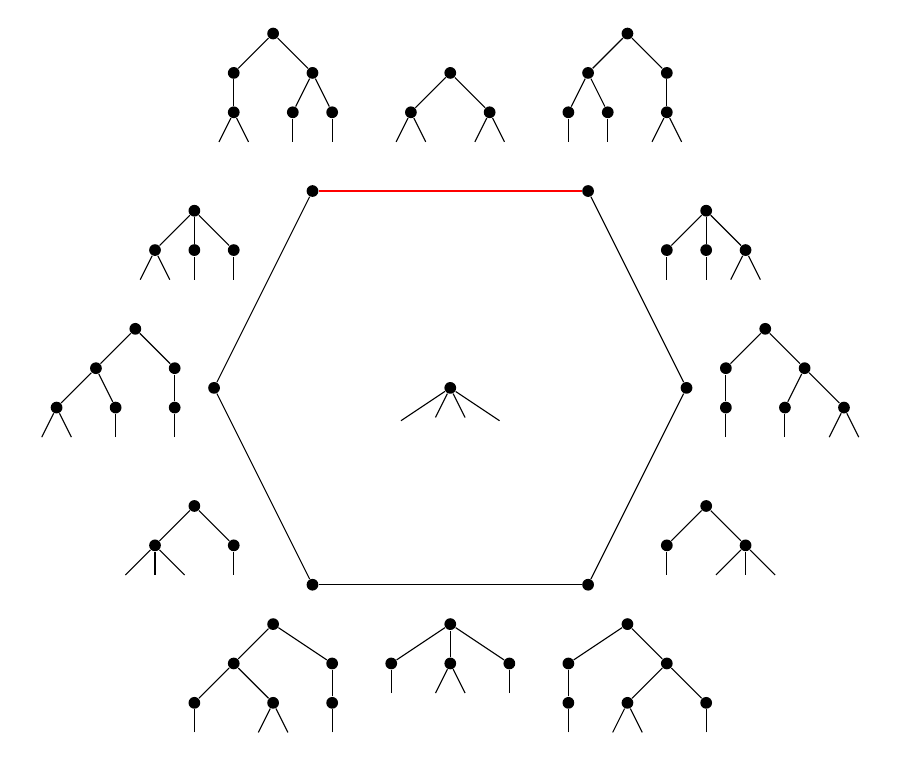
\begin{tikzpicture}[scale = 0.5]
\node[] (a1) at (-2,0) {};
\node[] (a2) at (-1,0) {};
\node[] (a3) at (0,0) {};
\node[] (a4) at (1,0) {};
\node[circle, fill=black, inner sep=1.5pt] (b1) at (-1.5,1) {};
\node[circle, fill=black, inner sep=1.5pt] (b2) at (0,1) {};
\node[circle, fill=black, inner sep=1.5pt] (b3) at (1,1) {};
\node[circle, fill=black, inner sep=1.5pt] (c1) at (-1.5,2) {};
\node[circle, fill=black, inner sep=1.5pt] (c2) at (0.5,2) {};
\node[circle, fill=black, inner sep=1.5pt] (d1) at (-0.5,3) {};
\draw (a1) -- (b1);
\draw (a2) -- (b1);
\draw (a3) -- (b2);
\draw (a4) -- (b3);
\draw (b1) -- (c1);
\draw (b2) -- (c2);
\draw (b3) -- (c2);
\draw (c1) -- (d1);
\draw (c2) -- (d1);

\node[] (a'1) at (2.5,0) {};
\node[] (a'2) at (3.5,0) {};
\node[] (a'3) at (4.5,0) {};
\node[] (a'4) at (5.5,0) {};
\node[circle, fill=black, inner sep=1.5pt] (b'1) at (3,1) {};
\node[circle, fill=black, inner sep=1.5pt] (b'2) at (5,1) {};
\node[circle, fill=black, inner sep=1.5pt] (c'1) at (4,2) {};
\draw (a'1) -- (b'1);
\draw (a'2) -- (b'1);
\draw (a'3) -- (b'2);
\draw (a'4) -- (b'2);
\draw (b'1) -- (c'1);
\draw (b'2) -- (c'1);


\node[] (aa1) at (7,0) {};
\node[] (aa2) at (8,0) {};
\node[] (aa3) at (9,0) {};
\node[] (aa4) at (10,0) {};
\node[circle, fill=black, inner sep=1.5pt] (bb1) at (9.5,1) {};
\node[circle, fill=black, inner sep=1.5pt] (bb2) at (7,1) {};
\node[circle, fill=black, inner sep=1.5pt] (bb3) at (8,1) {};
\node[circle, fill=black, inner sep=1.5pt] (cc1) at (9.5,2) {};
\node[circle, fill=black, inner sep=1.5pt] (cc2) at (7.5,2) {};
\node[circle, fill=black, inner sep=1.5pt] (dd1) at (8.5,3) {};
\draw (aa1) -- (bb2);
\draw (aa2) -- (bb3);
\draw (aa3) -- (bb1);
\draw (aa4) -- (bb1);
\draw (bb1) -- (cc1);
\draw (bb2) -- (cc2);
\draw (bb3) -- (cc2);
\draw (cc1) -- (dd1);
\draw (cc2) -- (dd1);

\node[] (aa'1) at (9.5,-3.5) {};
\node[] (aa'2) at (10.5,-3.5) {};
\node[] (aa'3) at (11,-3.5) {};
\node[] (aa'4) at (12,-3.5) {};
\node[circle, fill=black, inner sep=1.5pt] (bb'1) at (9.5,-2.5) {};
\node[circle, fill=black, inner sep=1.5pt] (bb'2) at (10.5,-2.5) {};
\node[circle, fill=black, inner sep=1.5pt] (bb'3) at (11.5,-2.5) {};
\node[circle, fill=black, inner sep=1.5pt] (cc'1) at (10.5,-1.5) {};
\draw (aa'1) -- (bb'1);
\draw (aa'2) -- (bb'2);
\draw (aa'3) -- (bb'3);
\draw (aa'4) -- (bb'3);
\draw (bb'1) -- (cc'1);
\draw (bb'2) -- (cc'1);
\draw (bb'3) -- (cc'1);


\node[] (aaa1) at (11,-7.5) {};
\node[] (aaa2) at (12.5,-7.5) {};
\node[] (aaa3) at (13.5,-7.5) {};
\node[] (aaa4) at (14.5,-7.5) {};
\node[circle, fill=black, inner sep=1.5pt] (bbb1) at (14,-6.5) {};
\node[circle, fill=black, inner sep=1.5pt] (bbb2) at (11,-6.5) {};
\node[circle, fill=black, inner sep=1.5pt] (bbb3) at (12.5,-6.5) {};
\node[circle, fill=black, inner sep=1.5pt] (ccc1) at (13,-5.5) {};
\node[circle, fill=black, inner sep=1.5pt] (ccc2) at (11,-5.5) {};
\node[circle, fill=black, inner sep=1.5pt] (ddd1) at (12,-4.5) {};
\draw (aaa1) -- (bbb2);
\draw (aaa2) -- (bbb3);
\draw (aaa3) -- (bbb1);
\draw (aaa4) -- (bbb1);
\draw (bbb1) -- (ccc1);
\draw (bbb2) -- (ccc2);
\draw (bbb3) -- (ccc1);
\draw (ccc1) -- (ddd1);
\draw (ccc2) -- (ddd1);

\node[] (aaa'1) at (9.5,-11){};
\node[] (aaa'2) at (10.5,-11) {};
\node[] (aaa'3) at (11.5,-11) {};
\node[] (aaa'4) at (12.5,-11) {};
\node[circle, fill=black, inner sep=1.5pt] (bbb'1) at (9.5,-10) {};
\node[circle, fill=black, inner sep=1.5pt] (bbb'2) at (11.5,-10) {};
\node[circle, fill=black, inner sep=1.5pt] (ccc'1) at (10.5,-9) {};

\draw (aaa'1) -- (bbb'1);
\draw (aaa'2) -- (bbb'2);
\draw (aaa'3) -- (bbb'2);
\draw (aaa'4) -- (bbb'2);
\draw (bbb'1) -- (ccc'1);
\draw (bbb'2) -- (ccc'1);


\node[] (aaaa1) at (7,-15) {};
\node[] (aaaa2) at (8,-15) {};
\node[] (aaaa3) at (9,-15) {};
\node[] (aaaa4) at (10.5,-15) {};
\node[circle, fill=black, inner sep=1.5pt] (bbbb1) at (10.5,-14) {};
\node[circle, fill=black, inner sep=1.5pt] (bbbb2) at (7,-14) {};
\node[circle, fill=black, inner sep=1.5pt] (bbbb3) at (8.5,-14) {};
\node[circle, fill=black, inner sep=1.5pt] (cccc1) at (9.5,-13) {};
\node[circle, fill=black, inner sep=1.5pt] (cccc2) at (7,-13) {};
\node[circle, fill=black, inner sep=1.5pt] (dddd1) at (8.5,-12) {};
\draw (aaaa1) -- (bbbb2);
\draw (aaaa2) -- (bbbb3);
\draw (aaaa3) -- (bbbb3);
\draw (aaaa4) -- (bbbb1);
\draw (bbbb1) -- (cccc1);
\draw (bbbb2) -- (cccc2);
\draw (bbbb3) -- (cccc1);
\draw (cccc1) -- (dddd1);
\draw (cccc2) -- (dddd1);

\node[] (aaaa'1) at (2.5,-14) {};
\node[] (aaaa'2) at (3.5,-14) {};
\node[] (aaaa'3) at (4.5,-14) {};
\node[] (aaaa'4) at (5.5,-14) {};
\node[circle, fill=black, inner sep=1.5pt] (bbbb'1) at (2.5,-13) {};
\node[circle, fill=black, inner sep=1.5pt] (bbbb'2) at (4,-13) {};
\node[circle, fill=black, inner sep=1.5pt] (bbbb'3) at (5.5,-13) {};
\node[circle, fill=black, inner sep=1.5pt] (cccc'1) at (4,-12) {};
\draw (aaaa'1) -- (bbbb'1);
\draw (aaaa'2) -- (bbbb'2);
\draw (aaaa'3) -- (bbbb'2);
\draw (aaaa'4) -- (bbbb'3);
\draw (bbbb'1) -- (cccc'1);
\draw (bbbb'2) -- (cccc'1);
\draw (bbbb'3) -- (cccc'1);

\node[] (aaaaa1) at (-2.5,-15) {};
\node[] (aaaaa2) at (-1,-15) {};
\node[] (aaaaa3) at (0,-15) {};
\node[] (aaaaa4) at (1,-15) {};
\node[circle, fill=black, inner sep=1.5pt] (bbbbb1) at (1,-14) {};
\node[circle, fill=black, inner sep=1.5pt] (bbbbb2) at (-2.5,-14) {};
\node[circle, fill=black, inner sep=1.5pt] (bbbbb3) at (-0.5,-14) {};
\node[circle, fill=black, inner sep=1.5pt] (ccccc1) at (1,-13) {};
\node[circle, fill=black, inner sep=1.5pt] (ccccc2) at (-1.5,-13) {};
\node[circle, fill=black, inner sep=1.5pt] (ddddd1) at (-0.5,-12) {};
\draw (aaaaa1) -- (bbbbb2);
\draw (aaaaa2) -- (bbbbb3);
\draw (aaaaa3) -- (bbbbb3);
\draw (aaaaa4) -- (bbbbb1);
\draw (bbbbb1) -- (ccccc1);
\draw (bbbbb2) -- (ccccc2);
\draw (bbbbb3) -- (ccccc2);
\draw (ccccc1) -- (ddddd1);
\draw (ccccc2) -- (ddddd1);

\node[] (aaaaa'1) at (-4.5,-11) {};
\node[] (aaaaa'2) at (-3.5,-11) {};
\node[] (aaaaa'3) at (-2.5,-11) {};
\node[] (aaaaa'4) at (-1.5,-11) {};
\node[circle, fill=black, inner sep=1.5pt] (bbbbb'1) at (-3.5,-10) {};
\node[circle, fill=black, inner sep=1.5pt] (bbbbb'2) at (-1.5,-10) {};
\node[circle, fill=black, inner sep=1.5pt] (ccccc'1) at (-2.5,-9) {};
\draw (aaaaa'1) -- (bbbbb'1);
\draw (aaaaa'2) -- (bbbbb'1);
\draw (aaaaa'3) -- (bbbbb'1);
\draw (aaaaa'4) -- (bbbbb'2);
\draw (bbbbb'1) -- (ccccc'1);
\draw (bbbbb'2) -- (ccccc'1);


\node[] (aaa1) at (-6.5,-7.5) {};
\node[] (aaa2) at (-5.5,-7.5) {};
\node[] (aaa3) at (-4.5,-7.5) {};
\node[] (aaa4) at (-3,-7.5) {};
\node[circle, fill=black, inner sep=1.5pt] (bbb1) at (-3,-6.5) {};
\node[circle, fill=black, inner sep=1.5pt] (bbb2) at (-6,-6.5) {};
\node[circle, fill=black, inner sep=1.5pt] (bbb3) at (-4.5,-6.5) {};
\node[circle, fill=black, inner sep=1.5pt] (ccc1) at (-3,-5.5) {};
\node[circle, fill=black, inner sep=1.5pt] (ccc2) at (-5,-5.5) {};
\node[circle, fill=black, inner sep=1.5pt] (ddd1) at (-4,-4.5) {};
\draw (aaa1) -- (bbb2);
\draw (aaa2) -- (bbb2);
\draw (aaa3) -- (bbb3);
\draw (aaa4) -- (bbb1);
\draw (bbb1) -- (ccc1);
\draw (bbb2) -- (ccc2);
\draw (bbb3) -- (ccc2);
\draw (ccc1) -- (ddd1);
\draw (ccc2) -- (ddd1);

\node[] (aaa''1) at (-4,-3.5) {};
\node[] (aaa''2) at (-3,-3.5) {};
\node[] (aaa''3) at (-2.5,-3.5) {};
\node[] (aaa''4) at (-1.5,-3.5) {};
\node[circle, fill=black, inner sep=1.5pt] (bbb''1) at (-3.5,-2.5) {};
\node[circle, fill=black, inner sep=1.5pt] (bbb''2) at (-2.5,-2.5) {};
\node[circle, fill=black, inner sep=1.5pt] (bbb''3) at (-1.5,-2.5) {};
\node[circle, fill=black, inner sep=1.5pt] (ccc''1) at (-2.5,-1.5) {};
\draw (aaa''1) -- (bbb''1);
\draw (aaa''2) -- (bbb''1);
\draw (aaa''3) -- (bbb''2);
\draw (aaa''4) -- (bbb''3);
\draw (bbb''1) -- (ccc''1);
\draw (bbb''2) -- (ccc''1);
\draw (bbb''3) -- (ccc''1);

\node[] (aaa'''1) at (2.5,-7) {};
\node[] (aaa'''2) at (3.5,-7) {};
\node[] (aaa'''3) at (4.5,-7) {};
\node[] (aaa'''4) at (5.5,-7) {};
\node[circle, fill=black, inner sep=1.5pt] (bbb'''1) at (4,-6) {};
\draw (aaa'''1) -- (bbb'''1);
\draw (aaa'''2) -- (bbb'''1);
\draw (aaa'''3) -- (bbb'''1);
\draw (aaa'''4) -- (bbb'''1);

\node[circle, fill=black, inner sep=1.5pt, label=below left:$$] (w1) at (0.5,-1) {$$};
\node[circle, fill=black, inner sep=1.5pt, label=below left:$$] (w2) at (7.5,-1) {$$};
\node[circle, fill=black, inner sep=1.5pt, label=below left:$$] (w3) at (10,-6) {$$};
\node[circle, fill=black, inner sep=1.5pt, label=below left:$$] (w4) at (7.5,-11) {$$};
\node[circle, fill=black, inner sep=1.5pt, label=below left:$$] (w5) at (0.5,-11) {$$};
\node[circle, fill=black, inner sep=1.5pt, label=below left:$$] (w6) at (-2,-6) {$$};
\node[] (w7) at (4,-1) {$$};
\draw (w1)[color=red] -- (w2);
\draw (w2) -- (w3);
\draw (w3) -- (w4);
\draw (w4) -- (w5);
\draw (w5) -- (w6);
\draw (w6) -- (w1);



\end{tikzpicture} \end{center}

\hfill

\hfill

The associahedron $\mathbf{K}_{2}$ with $A$-trees on $4$ leaves
attached to each $k$-cell of $\mathbf{K}_{2}$:

\begin{center}\begin{tikzpicture}[scale = 0.5]

\node[] (a'1) at (2.5,0) {};
\node[] (a'2) at (3.5,0) {};
\node[] (a'3) at (4.5,0) {};
\node[] (a'4) at (5.5,0) {};
\node[circle, fill=black, inner sep=1.5pt] (b'1) at (3,1) {};
\node[circle, fill=black, inner sep=1.5pt] (b'2) at (5,1) {};
\node[circle, fill=black, inner sep=1.5pt] (c'1) at (4,2) {};
\draw (a'1) -- (b'1);
\draw (a'2) -- (b'1);
\draw (a'3) -- (b'2);
\draw (a'4) -- (b'2);
\draw (b'1) -- (c'1);
\draw (b'2) -- (c'1);


\node[] (aa'3) at (9,-3.5) {};
\node[] (aa'4) at (10,-3.5) {};
\node[] (bb'1) at (7.5,-2.5) {};
\node[] (bb'2) at (8.5,-2.5) {};
\node[circle, fill=black, inner sep=1.5pt] (bb'3) at (9.5,-2.5) {};
\node[circle, fill=black, inner sep=1.5pt] (cc'1) at (8.5,-1.5) {};
\draw (aa'3) -- (bb'3);
\draw (aa'4) -- (bb'3);
\draw (bb'1) -- (cc'1);
\draw (bb'2) -- (cc'1);
\draw (bb'3) -- (cc'1);


\node[] (aaa3) at (13.5,-7.5) {};
\node[] (aaa4) at (14.5,-7.5) {};
\node[circle, fill=black, inner sep=1.5pt] (bbb1) at (14,-6.5) {};
\node[] (bbb3) at (12.5,-6.5) {};
\node[circle, fill=black, inner sep=1.5pt] (ccc1) at (13,-5.5) {};
\node[] (ccc2) at (11.5,-5.5) {};
\node[circle, fill=black, inner sep=1.5pt] (ddd1) at (12,-4.5) {};
\draw (aaa3) -- (bbb1);
\draw (aaa4) -- (bbb1);
\draw (bbb1) -- (ccc1);
\draw (bbb3) -- (ccc1);
\draw (ccc1) -- (ddd1);
\draw (ccc2) -- (ddd1);

\node[] (aaa'2) at (10.5,-11) {};
\node[] (aaa'3) at (11.5,-11) {};
\node[] (aaa'4) at (12.5,-11) {};
\node[] (bbb'1) at (9.5,-10) {};
\node[circle, fill=black, inner sep=1.5pt] (bbb'2) at (11.5,-10) {};
\node[circle, fill=black, inner sep=1.5pt] (ccc'1) at (10.5,-9) {};

\draw (aaa'2) -- (bbb'2);
\draw (aaa'3) -- (bbb'2);
\draw (aaa'4) -- (bbb'2);
\draw (bbb'1) -- (ccc'1);
\draw (bbb'2) -- (ccc'1);


\node[] (aaaa2) at (8,-15) {};
\node[] (aaaa3) at (9,-15) {};
\node[] (aaaa4) at (10.5,-15) {};
\node[circle, fill=black, inner sep=1.5pt] (bbbb1) at (10.5,-14) {};
\node[circle, fill=black, inner sep=1.5pt] (bbbb3) at (8.5,-14) {};
\node[circle, fill=black, inner sep=1.5pt] (cccc1) at (9.5,-13) {};
\node[] (cccc2) at (7.5,-13) {};
\node[circle, fill=black, inner sep=1.5pt] (dddd1) at (8.5,-12) {};
\draw (aaaa2) -- (bbbb3);
\draw (aaaa3) -- (bbbb3);
\draw (aaaa4) -- (bbbb1);
\draw (bbbb1) -- (cccc1);
\draw (bbbb3) -- (cccc1);
\draw (cccc1) -- (dddd1);
\draw (cccc2) -- (dddd1);

\node[] (aaaa'2) at (3.5,-14) {};
\node[] (aaaa'3) at (4.5,-14) {};
\node[] (bbbb'1) at (2.5,-13) {};
\node[circle, fill=black, inner sep=1.5pt] (bbbb'2) at (4,-13) {};
\node[] (bbbb'3) at (5.5,-13) {};
\node[circle, fill=black, inner sep=1.5pt] (cccc'1) at (4,-12) {};
\draw (aaaa'2) -- (bbbb'2);
\draw (aaaa'3) -- (bbbb'2);
\draw (bbbb'1) -- (cccc'1);
\draw (bbbb'2) -- (cccc'1);
\draw (bbbb'3) -- (cccc'1);

\node[] (aaaaa1) at (-2.5,-15) {};
\node[] (aaaaa2) at (-1,-15) {};
\node[] (aaaaa3) at (0,-15) {};
\node[circle, fill=black, inner sep=1.5pt] (bbbbb2) at (-2.5,-14) {};
\node[circle, fill=black, inner sep=1.5pt] (bbbbb3) at (-0.5,-14) {};
\node[] (ccccc1) at (0.5,-13) {};
\node[circle, fill=black, inner sep=1.5pt] (ccccc2) at (-1.5,-13) {};
\node[circle, fill=black, inner sep=1.5pt] (ddddd1) at (-0.5,-12) {};
\draw (aaaaa1) -- (bbbbb2);
\draw (aaaaa2) -- (bbbbb3);
\draw (aaaaa3) -- (bbbbb3);
\draw (bbbbb2) -- (ccccc2);
\draw (bbbbb3) -- (ccccc2);
\draw (ccccc1) -- (ddddd1);
\draw (ccccc2) -- (ddddd1);

\node[] (aaaaa'1) at (-4.5,-11) {};
\node[] (aaaaa'2) at (-3.5,-11) {};
\node[] (aaaaa'3) at (-2.5,-11) {};
\node[circle, fill=black, inner sep=1.5pt] (bbbbb'1) at (-3.5,-10) {};
\node[] (bbbbb'2) at (-1.5,-10) {};
\node[circle, fill=black, inner sep=1.5pt] (ccccc'1) at (-2.5,-9) {};
\draw (aaaaa'1) -- (bbbbb'1);
\draw (aaaaa'2) -- (bbbbb'1);
\draw (aaaaa'3) -- (bbbbb'1);
\draw (bbbbb'1) -- (ccccc'1);
\draw (bbbbb'2) -- (ccccc'1);


\node[] (aaa1) at (-6.5,-7.5) {};
\node[] (aaa2) at (-5.5,-7.5) {};
\node[] (aaa3) at (-4.5,-7.5) {};
\node[circle, fill=black, inner sep=1.5pt] (bbb2) at (-6,-6.5) {};
\node[circle, fill=black, inner sep=1.5pt] (bbb3) at (-4.5,-6.5) {};
\node[] (ccc1) at (-3,-5.5) {};
\node[circle, fill=black, inner sep=1.5pt] (ccc2) at (-5,-5.5) {};
\node[circle, fill=black, inner sep=1.5pt] (ddd1) at (-4,-4.5) {};
\draw (aaa1) -- (bbb2);
\draw (aaa2) -- (bbb2);
\draw (aaa3) -- (bbb3);
\draw (bbb2) -- (ccc2);
\draw (bbb3) -- (ccc2);
\draw (ccc1) -- (ddd1);
\draw (ccc2) -- (ddd1);

\node[] (aaa''1) at (-2,-3.5) {};
\node[] (aaa''2) at (-1,-3.5) {};
\node[circle, fill=black, inner sep=1.5pt] (bbb''1) at (-1.5,-2.5) {};
\node[] (bbb''2) at (-0.5,-2.5) {};
\node[] (bbb''3) at (0.5,-2.5) {};
\node[circle, fill=black, inner sep=1.5pt] (ccc''1) at (-0.5,-1.5) {};
\draw (aaa''1) -- (bbb''1);
\draw (aaa''2) -- (bbb''1);
\draw (bbb''1) -- (ccc''1);
\draw (bbb''2) -- (ccc''1);
\draw (bbb''3) -- (ccc''1);

\node[] (aaa'''1) at (2.5,-7) {};
\node[] (aaa'''2) at (3.5,-7) {};
\node[] (aaa'''3) at (4.5,-7) {};
\node[] (aaa'''4) at (5.5,-7) {};
\node[circle, fill=black, inner sep=1.5pt] (bbb'''1) at (4,-6) {};
\draw (aaa'''1) -- (bbb'''1);
\draw (aaa'''2) -- (bbb'''1);
\draw (aaa'''3) -- (bbb'''1);
\draw (aaa'''4) -- (bbb'''1);

\node[circle, fill=black, inner sep=1.5pt, label=below left:$$] (w3) at (10,-6) {$$};
\node[circle, fill=black, inner sep=1.5pt, label=below left:$$] (w4) at (7.5,-11) {$$};
\node[circle, fill=black, inner sep=1.5pt, label=below left:$$] (w5) at (0.5,-11) {$$};
\node[circle, fill=black, inner sep=1.5pt, label=below left:$$] (w6) at (-2,-6) {$$};
\node[circle, fill=black, inner sep=1.5pt, label=below left:$$] (w7) at (4,-1) {$$};

\draw (w7) -- (w3);
\draw (w3) -- (w4);
\draw (w4) -- (w5);
\draw (w5) -- (w6);
\draw (w3) -- (w7);
\draw (w6) -- (w7);


\end{tikzpicture} \end{center}

~~~In this section, we count the number of $k$-cells on the $n$-dimensional
permutohedron $\mathbf{P}_{n}$ which collapse to a $0$-cell on an
associahedron $K_{n-1}$. 

\begin{lemma} Let $x_{1},\dots,x_{m},y_{1},\dots,y_{n}$ be elements
of some set. Then there are ${m \choose k}{m+n-k \choose m}$ ways
of ordering these elements such that $x_{i}<x_{j}$ and $y_{i}<y_{j}$
whenever $i<j$, and $k$ of the $y_{i}$'s are tied with $k$ of
the $x_{j}'s$. \end{lemma}

\begin{proof} There are ${m \choose k}$ ways to select $k$ of the
$x_{i}$'s to be tied with and ${m+n-k \choose m}$ ways of rearranging
everything else. \end{proof}

\begin{example} Here is a way to order the list $x_{1},x_{2},x_{3},x_{4},x_{5},y_{1},y_{2},y_{3},y_{4}$
such that $x_{i}<x_{j}$ and $y_{i}<y_{j}$ whenever $i<j$, and $2$
of the $y_{i}$'s are tied with $2$ of the $x_{j}'s$:
\[
x_{1}<x_{2}<y_{1}<x_{3}=y_{2}<y_{3}<x_{4}=y_{4}<x_{5}
\]
 \end{example}

~~~Let $T$ be a binary $A$-tree, $L$ be the subtree whose root
is the left child of the root of $T$, and $R$ be the subtree whose
root is the right child of the root of $T$. Let $n_{T}$, $n_{L},$
and $n_{R}$ be the number of internal nodes of each tree respectively.
Finally, let $P_{k}(T)$, $P_{k}(L)$, and $P_{k}(R)$ be the number
of $k$-cells on the permutohedron which collapse to the $0$-cell
on the associahedron which corresponds to each binary tree respectively.
Then 

\[
\sum_{i=0}^{k}\sum_{j=0}^{k-i}{n_{L}-i \choose k-i-j}{n_{L}+n_{R}-k \choose n_{L}-i}P_{i}(L)P_{j}(R)=P_{k}(T)
\]

\begin{center}\begin{tikzpicture}

\node[] (a1) at (0,0) {};
\node[] (a2) at (1,0) {};
\node[] (a3) at (2,0) {};
\node[] (a4) at (3,0) {};
\node[] (a5) at (4,0) {};
\node[] (a6) at (5,0) {};

\node[circle, fill=black, inner sep=1.5pt, label=below left:$$] (b1) at (0.5,1) {};
\node[circle, fill=black, inner sep=1.5pt, label=below left:$$] (b2) at (1.25,2) {};
\node[circle, fill=black, inner sep=1.5pt, label=below left:$$] (b3) at (2.15,3) {};
\node[circle, fill=black, inner sep=1.5pt, label=below left:$$] (b4) at (4,1) {};
\node[circle, fill=black, inner sep=1.5pt, label=below left:$$] (b5) at (5,1) {};
\node[circle, fill=black, inner sep=1.5pt, label=below left:$$] (b6) at (6,1) {};
\node[circle, fill=black, inner sep=1.5pt, label=below left:$$] (b7) at (7,1) {};

\node[circle, fill=black, inner sep=1.5pt, label=below left:$$] (c1) at (0.5,2) {};
\node[circle, fill=black, inner sep=1.5pt, label=below left:$$] (c2) at (2.5,2) {};
\node[circle, fill=black, inner sep=1.5pt, label=below left:$$] (c3) at (4,2) {};
\node[circle, fill=black, inner sep=1.5pt, label=below left:$$] (c4) at (5,2) {};
\node[circle, fill=black, inner sep=1.5pt, label=below left:$$] (c5) at (6,2) {};
\node[circle, fill=black, inner sep=1.5pt, label=below left:$$] (c6) at (7,2) {};

\node[circle, fill=black, inner sep=1.5pt, label=below left:$$] (d1) at (0.5,3) {};
\node[circle, fill=black, inner sep=1.5pt, label=below left:$$] (d2) at (2.5,3) {};
\node[circle, fill=black, inner sep=1.5pt, label=below left:$$] (d3) at (4,3) {};
\node[circle, fill=black, inner sep=1.5pt, label=below left:$$] (d4) at (5,3) {};
\node[circle, fill=black, inner sep=1.5pt, label=below left:$$] (d5) at (6.5,3) {};

\node[circle, fill=black, inner sep=1.5pt, label=below left:$$] (e1) at (0.5,4) {};
\node[circle, fill=black, inner sep=1.5pt, label=below left:$$] (e2) at (2.5,4) {};
\node[circle, fill=black, inner sep=1.5pt, label=below left:$$] (e3) at (4.5,4) {};
\node[circle, fill=black, inner sep=1.5pt, label=below left:$$] (e4) at (6.5,4) {};

\node[circle, fill=black, inner sep=1.5pt, label=below left:$$] (f1) at (1.5,5) {};
\node[circle, fill=black, inner sep=1.5pt, label=below left:$$] (f2) at (4.5,5) {};
\node[circle, fill=black, inner sep=1.5pt, label=below left:$$] (f3) at (6.5,5) {};

\node[circle, fill=black, inner sep=1.5pt, label=below left:$$] (g1) at (1.5,6) {};
\node[circle, fill=black, inner sep=1.5pt, label=below left:$$] (g2) at (5.5,6) {};

\node[circle, fill=black, inner sep=1.5pt, label=below left:$$] (h1) at (3.5,7) {};


\draw (a1) -- (b1);
\draw (a2) -- (b2);
\draw (a3) -- (b3);
\draw (a4) -- (b3);
\draw (a5) -- (b4);
\draw (a6) -- (b5);
\draw (a7) -- (b6);
\draw (a8) -- (b7);

\draw (b1) -- (c1);
\draw (b2) -- (c1);
\draw (b3) -- (c2);
\draw (b4) -- (c3);
\draw (b5) -- (c4);
\draw (b6) -- (c5);
\draw (b7) -- (c6);

\draw (c1) -- (d1);
\draw (c2) -- (d2);
\draw (c3) -- (d3);
\draw (c4) -- (d4);
\draw (c5) -- (d5);
\draw (c6) -- (d5);

\draw (d1) -- (e1);
\draw (d2) -- (e2);
\draw (d3) -- (e3);
\draw (d4) -- (e3);
\draw (d5) -- (e4);

\draw (e1) -- (f1);
\draw (e2) -- (f1);
\draw (e3) -- (f2);
\draw (e4) -- (f3);

\draw (f1) -- (g1);
\draw (f2) -- (g2);
\draw (f3) -- (g2);

\draw (g1) -- (h1);
\draw (g2) -- (h1);

\end{tikzpicture} \end{center}

We want to count the number of nondegenerate $P$-trees which collapse
to an $A$-tree. 

\[
d_{2}((g_{1}g_{2})(g_{3})(g_{4}g_{5}))((g_{6}g_{7})(g_{8}g_{9}))=(g_{1}g_{2}g_{3}g_{4}g_{5})(g_{6}g_{7}g_{8}g_{9})-(g_{1}g_{2})(g_{3})(g_{4}g_{5})(g_{6}g_{7})(g_{8}g_{9})
\]
\[
\prod_{i\in\mathbb{N}}g_{i}
\]
\[
\prod_{j\in\mathbb{N}}\left(\prod_{g_{ij}\in G}g_{ij}\right)
\]
\[
\prod_{k\in\mathbb{N}}\left(\prod_{j\in\mathbb{N}}\left(\prod_{i\in\mathbb{N}}g_{ijk}\right)\right)
\]
\[
\left(\left(g_{111}g_{211}g_{311}g_{411}\right)\left(g_{121}g_{221}g_{321}\right)\right)\left(\left(g_{112}\right)\left(g_{122}g_{222}g_{322}g_{422}\right)\left(g_{132}g_{232}\right)\right)\left(\left(g_{113}g_{213}\right)\right)
\]
\[
\prod_{k=1}^{3}\left(\prod_{j=1}^{2}\left(\prod_{i=1}^{4}g_{ijk}\right)\right)=\left(\left(g_{111}g_{211}g_{311}g_{411}\right)\left(g_{121}g_{221}g_{321}g_{421}\right)\right)\left(\left(g_{112}g_{212}g_{312}g_{412}\right)\left(g_{122}g_{222}g_{322}g_{422}\right)\right)\left(\left(g_{113}g_{213}g_{313}g_{413}\right)\left(g_{123}g_{223}g_{323}g_{423}\right)\right)
\]
\[
d_{2}\prod_{k\in\mathbb{N}}\left(\prod_{j\in\mathbb{N}}\left(\prod_{i\in\mathbb{N}}g_{ijk}\right)\right)=\prod_{k\in\mathbb{N}}\left(\prod_{j\in\mathbb{N}}\prod_{i\in\mathbb{N}}g_{ijk}\right)-\prod_{k\in\mathbb{N}}\prod_{j\in\mathbb{N}}\left(\prod_{i\in\mathbb{N}}g_{ijk}\right)
\]

\begin{center}\begin{tikzpicture}


\node[circle, fill=black, inner sep=1.5pt, label=left:$ (1)(2)(3)(5)(6)(4)$] (a) at (-11,11) {};
\node[circle, fill=black, inner sep=1.5pt, label=above right:$ (1)(2)(5)(3)(6)(4)$] (b) at (-8,8) {};
\node[circle, fill=black, inner sep=1.5pt, label=below left:$ (1)(2)(5)(6)(3)(4)$] (c) at (-10,6) {};
\node[circle, fill=black, inner sep=1.5pt, label=above right:$ (1)(5)(2)(6)(3)(4)$] (d) at (-2,7) {};
\node[circle, fill=black, inner sep=1.5pt, label=right:$ (1)(2)(5)(6)(3)(4)$] (e) at (-4,5) {};
\node[circle, fill=black, inner sep=1.5pt, label=above left:$ (5)(1)(2)(6)(3)(4)$] (f) at (-5,6) {};
\node[circle, fill=black, inner sep=1.5pt, label=left:$ (1)(2)(5)(6)(3)(4)$] (g) at (-7,4) {};
\node[circle, fill=black, inner sep=1.5pt, label=below left:$ (5)(1)(2)(6)(3)(4)$] (h) at (-4,1) {};
\node[circle, fill=black, inner sep=1.5pt, label=right:$ (1)(5)(6)(2)(3)(4)$] (i) at (-1,2) {};
\node[circle, fill=black, inner sep=1.5pt, label=right:$ (5)(6)(1)(2)(3)(4)$] (j) at (2,0) {};

\draw (a) -- (b);
\draw (b) -- (c);
\draw (b) -- (d);
\draw (d) -- (e);
\draw (c) -- (e);
\draw (d) -- (f);
\draw (f) -- (g);
\draw (e) -- (g);
\draw (h) -- (g);
\draw (i) -- (e);
\draw (i) -- (h);
\draw (h) -- (j);


\end{tikzpicture} \end{center}
\end{document}
